\documentclass[12pt]{article}
\usepackage[T1]{fontenc}
\usepackage[utf8]{inputenc}
\usepackage[sfdefault]{carlito}
\renewcommand{\baselinestretch}{1.5}

\usepackage{float}
%\usepackage[a4paper,hmargin=1.5cm,vmargin=2cm]{geometry}
\usepackage[a4paper,left=3.5cm,right=2.5cm,top=2.5cm,bottomright=2.5cm]{geometry}
\usepackage{graphicx}
\usepackage{amsfonts}
\usepackage{textcomp}
\usepackage{hyperref}
\usepackage{array}
\usepackage{tabularx}
\usepackage{mathtools}
\usepackage{longtable}
\usepackage{enumitem}
\usepackage{caption}

\renewcommand{\figurename}{Fig.}
% set custom numeration of figures to be x.y, where x is section number
\renewcommand{\thefigure}{\arabic{section}.\arabic{figure}}
% set custom numeration of tables to be x.y, where x is section number
\renewcommand{\thetable}{\arabic{section}.\arabic{table}}

%%%%%%%%%%%%%%%%%%%%%%%%%%%%%%%%%%%%%%%%%%%%%%%%%%%%%%%%%%%%%%%%%%%%%%%%%%%%%%%%
% Configure code listings
% $ tlmgr install mdframed needspace chngcntr

\usepackage{mdframed}
\usepackage[]{listings}
\renewcommand*{\lstlistlistingname}{List of Listings}
% by default the listings are numered as: Listing 1, Listing 2,
% the command below replaces the "Listing" to an empty string
% \renewcommand{\lstlistingname}{ }

\usepackage{chngcntr}


\usepackage{xcolor}
\DeclareCaptionFont{white}{\color{white}}

\DeclareCaptionFormat{listing}{%
  \parbox{\textwidth}{
    \colorbox{gray}{
      %\parbox{\textwidth}{\color{white}Listing \arabic{section}.#1#2#3}
      \parbox{\textwidth}{#1#2#3}
    }

  }
}
%\captionsetup[lstlisting]{
%  format=listing,
%  labelfont=white,
%  textfont=white,
%  justification=centering,
%  % singlelinecheck=off means that the justification setting is used even when the caption is only a single line long.
%  singlelinecheck=off
%}
\lstset{
  basicstyle=\tiny,frame=lrtb,
  xleftmargin=1cm,
  %xleftmargin=\fboxsep,xrightmargin=-\fboxsep,
  captionpos=b
}

%%%%%%%%%%%%%%%%%%%%%%%%%%%%%%%%%%%%%%%%%%%%%%%%%%%%%%%%%%%%%%%%%%%%%%%%%%%%%%%%

% parsep is interlinia
\setitemize{noitemsep,topsep=5pt,parsep=0pt,partopsep=0pt}
\setenumerate{noitemsep,topsep=5pt,parsep=0pt,partopsep=0pt}

\usepackage[backend=bibtex,sorting=ydnt]{biblatex}
\setlength\bibitemsep{0pt}
\bibliography{thesis-tex/bibliography.bib}


\usepackage{wrapfig}
\graphicspath{{figures/}}

\title{
{\small Ewa Czechowska } \\
\bf\textit{ Master’s Thesis - TODO replace me } \\
\vspace{4cm}}
\date{\today}

\begin{document}
\numberwithin{lstlisting}{section}

\maketitle
~\vspace{8cm}
\newpage

\tableofcontents
\newpage
\begin{abstract}
{\scriptsize The presented master's thesis aims to deploy Kubernetes cluster on AWS cloud, in a production environment, using different deployment methods. The production environment is defined as an environment which satisfies selected requirements. The nine requirements were selected, including among others central logging, high availability and automation.}

{\scriptsize Two deployment methods were chosen: using kops and using eksctl. The methods are first theoretically research and described. Then, they are used in the empirical part to deploy Kubernetes clusters. The methods are a~great help and they facilitate the cluster deployment.}

{\scriptsize \textbf{These two methods of Kubernetes cluster deployment were compared} using several comparison criteria. The criteria contained, among others: time, cost and the verdict whether a deployment method can satisfy all the production environment requirements. The conclusion was that each method can be used for different use cases. For example: kops allows more configuration, whereas eksctl is easier to configure. Kops method was deemed faster (in relation to cluster operations) and cheaper.}

{\scriptsize \textbf{Keywords:} Kubernetes, Amazon Web Services (AWS), Amazon Elastic Kubernetes Service (EKS), eksctl, kops, deployment, operations automation.}

\\
\begin{center}
\textbf{Streszczenie}
\end{center}

{\scriptsize Celem tej pracy magisterskiej jest zainstalowanie i skonfigurowanie klustra Kubernetes na chmurze AWS, w~środowisku produkcyjnym, wykorzystując różne metody. Środowisko produkcyjne zdefiniowano jako takie środowisko, które spełnia wybrane wymagania. Wyselekcjonowano dziewięć wymagań, m. in.: centralny system logowania, High Availability oraz automatyzację operacji.}

{\scriptsize Wybrano dwie metody wdrażana klustra Kubernetes: używając programu kops oraz programu eksctl. Metody te zostały najpierw poznane i opisane teoretycznie. Następnie, wykorzystano je w empirycznej części pracy. Obie metody stanowiły wielką pomoc w instalowaniu i konfiguracji klustra.}

{\scriptsize Następnie, \textbf{te dwie wybrane metody wdrażana klustra Kubernetes porównano}, wykorzystując parę kryteriów. Kryteria te dotyczyły m. in.: czasu, kosztu, sprawdzenia, czy każda z metod spełnia wybrane wymogi środowiska produkcyjnego. Po tym badaniu wysnuto wniosek, że każda z wybranych metod może być użyta w zależności od potrzeb. Na przykład: posługując się programem kops, dostępne jest więcej opcji konfigurujących kluster, a natomiast używając eksctl - konfiguracja jest łatwiejsza. Metoda używająca kops okazała się szybsza (jeśli chodzi o czas wykonywania operacji typu: stworzenie, przetestowanie, usunięcie klustra) i tańsza.}


{\scriptsize \textbf{Słowa kluczowe:} Kubernetes, Amazon Web Services (AWS), Amazon Elastic Kubernetes Service (EKS), eksctl, kops, deployment, automatyzacja operacji.}
\end{abstract}

\newpage

% 1
\setcounter{figure}{0}
\setcounter{table}{0}
\setcounter{lstlisting}{0}
\section{Introduction}

% this should take 2 or 3 pages;
% the subsections are not mandatory

\subsection{Topic and problem description}

Microservices, Continuous Integration and Delivery, Docker, DevOps, Infrastructure as Code - these are the current trends and buzzwords in the technological world of 2020. A popular tool which can \textbf{facilitate the deployment and maintenance of microservices is Kubernetes}. Kubernetes is a platform for running containerized applications, for example: microservices. The first part of the problem, which this thesis is trying to solve is: \textbf{how to deploy Kubernetes itself}. The second part is: how to ensure that the deployment fulfills the needs of a production environment.

Any application may comprise several components, for example: a backend server, a frontend server, database. It is common knowledge, that deploying an application to a production environment, should obey a set of guidelines. It should be easy to view all the log messages generated by each of the components of the application, the application should be reachable for its end users and also, it would be nice if in a case of any component failure - that component should be available despite the failure. \textbf{Kubernetes facilitates satisfying such requirements. But, the aim of this thesis is to ensure such requirements for Kubernetes itself}. A set of requirements will be selected. Then, several ideas will be provided on how to meet each of the chosen requirements.

\textbf{There are plenty methods of Kubernetes cluster deployment. Many will be described}. The methods differ in relation to: how much customization they offer, which clouds they support, how much they cost. Some of the methods has existed since the Kubernetes was created, the other ones, like AWS EKS, has been invented later. The latter methods are harder to find in books tackling the Kubernetes deployment task, but there are other sources which explain how to use them (mostly: official documentation of the methods and blog posts).

There exist sources which compare several methods of Kubernetes cluster deployment. But, they are either non-formal sources (e.g. blog posts or Internet tutorials) or they do not compare the two methods selected in this thesis or they do not consider the production environment. Therefore, \textbf{this thesis has the opportunity to offer some novelty}.

\subsection{Aim and scope of this study}


Nowadays, the world is full of choices. The technology is exuberant. However, time, as our resource, is limited. Thus, it is often advisable to use an already existing solution instead of inventing our own. It is even better if there are many such solutions. The presented Master's thesis aims \textbf{to compare two methods of deploying a Kubernetes cluster}. Both of the methods concern AWS cloud. AWS cloud was chosen mainly because of its wide popularity and the range of provided services. Besides the two chosen methods of deployment, there are many more, including the DIY method and deploying on-premises.

This thesis attempts \textbf{to stipulate the requirements of a production environment}. Then, the requirements are used as comparison criteria to help assess the two methods of deployment. It is expected that one method could be easier to use than the other but also a method could be insufficient to satisfy all the production environment requirements. Furthermore, other criteria will be used, such as: cost of both methods and amount of problems encountered.

It is intended, that this work should \textbf{focus on the practical aspect of a Kubernetes cluster deployment}. The limitations and known issues of both methods are going to be described. Therefore, the thesis might be helpful to the engineers or consultants who are responsible for Kubernetes cluster deployment.

There are already some literature sources that compare chosen methods of Kubernetes cluster deployment. However, they are not constructed in a scientific, formal form (they are either blog posts or tutorials available in the Internet) or they do not consider a production environment.

\subsection{Structure of this thesis}

The presented thesis is divided into seven chapters.

The first chapter is \textbf{an introduction}. It describes briefly the topic and the problem. Then, it includes aim and scope of this study. And then, the structure of this study is presented.

The second chapter focuses on \textbf{basic information concerning: microservices, DevOps, Docker and Kubernetes}. Furthermore, AWS cloud is described there. The chapter ends with stipulating the requirements of a production deployment.

In the next, third, chapter \textbf{the most popular methods of Kubernetes cluster deployment are described}. The two methods that will be compared in the later part are also included.

The fourth chapter is a practical one. It provides \textbf{planning and designing of the production deployment} which will be conducted later in the thesis. Some important decisions are taken here, for example: which Kubernetes version to use or which tools to use.

Then, the fifth chapter \textbf{refers to code} and it is the core part of this Master's thesis. It provides \textbf{the steps that were used to deploy Kubernetes clusters on AWS, using two methods}:
\begin{enumerate}
\item deployment on AWS EKS service,
\item deployment with Kops on AWS EC2 instances.
\end{enumerate}
Anyone following these steps should be capable to recreate the same Kubernetes clusters as described here and thus, it should be possible to draw the same conclusions as the author of this thesis did. Furthermore, all the encountered problems and suggested solutions are provided.

The sixth chapter \textbf{presents the comparison} of the two deployment methods using chosen comparison criteria. Each subsection of this chapter deals with a single comparison criterion.

Finally, the last, seventh, chapter offers \textbf{the summary}, briefly describes the lessons learned and also provides some ideas for future work.

\newpage

% 2
\setcounter{figure}{0}
\setcounter{table}{0}
\setcounter{lstlistings}{0}
\section{From microservices to automated orchestration}
\textit{This chapter serves as an introduction to microservices, DevOps, Docker, Kubernetes and AWS. It ends with stipulating the requirements of a production deployment.}

\subsection{Microservices, DevOps, Continuous Delivery and Infrastructure as Code}
\textit{This subchapter attempts to briefly explain a set of terms which will be used throughout this Master's thesis.}


\subsubsection{Microservices}
Microservices may be defined as a \textbf{cloud-native architecture} which aim is to provide software systems as a package of small services. Each of these small services should be \textbf{independently deployable} and also each of them could utilize a different technological stack and platform. The services run in separate processes and communicate with each other through mechanisms like: RESTful APIs \cite{article-micro-devops} because they utilize the language-agnostic protocol: HTTP \cite{book-pr-devops}.

Another definition of microservices is: "a microservice is simply \textbf{a self-contained service that does one thing}. If you put enough microservices together, you get an application" \cite{book-cndwk}.

Microservices are often presented as an alternative to and compared to \textbf{monoliths}. For instance, the author of "Practical DevOps" \cite{book-pr-devops} explains that, in comparison to monoliths, microservices have more integration points and suffer from a
higher possibility of failure. Furthermore, in \cite{book-cndwk} it is written that:
\begin{itemize}
\item monoliths are hard to scale, both in terms of code and also in terms of teams of people,
\item monoliths are easier to understand, because the code can be found in one place.
\end{itemize}

The schema presented in figure ~\ref{fig:microservices-vs-mono} should help to illustrate the difference between two software architecture styles.
\begin{figure}[H]
    \centering
    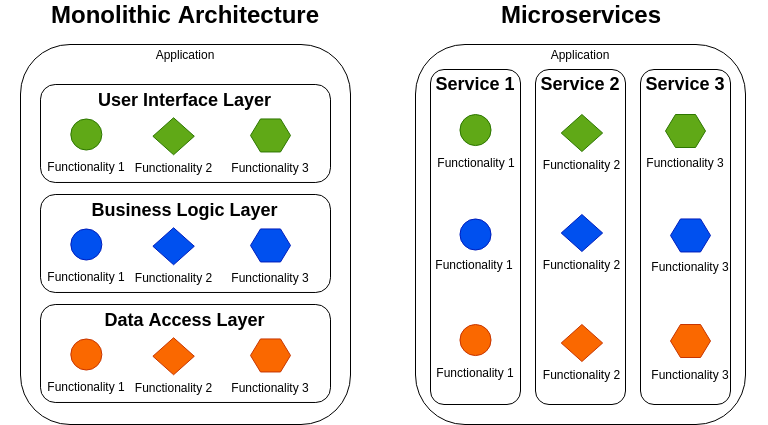
\includegraphics[width=10cm]{figures/microservices-vs-mono.png}
    \captionsetup{justification=centering,margin=2cm}
    \caption{The difference between two software architecture styles: monolith and microservices \cite{online-trans-mono-micro}}
    \label{fig:microservices-vs-mono}
\end{figure}

Microservices are not a panacea \cite{book-cndwk} and not a silver bullet \cite{article-micro-devops}, but in order to design a great software system, one should be acquainted with many solutions.

\subsubsection{DevOps}
\textbf{DevOps} and microservices have been both increasingly drawing attention since 2014, according to Google Trends. DevOps can be applied to both: monoliths and microservices, but using it for microservices promotes the importance of small teams. DevOps may be explained as a set of practices which aims \textbf{to decrease the time from the point of introducing a change to a point when the change is transferred to the production environment}. DevOps also focuses on maintaining the software quality in terms of both: code and the delivery process \cite{article-micro-devops}.

Moreover, DevOps can be defined as: "a movement to reduce barriers and friction between organizational silos - development, operations, and other stakeholders involved in planning, building, and running software". The definition continues, that even though the most visible aspect of DevOps may be technology, it is \textbf{culture, people and processes which have the most impact on flow and effectiveness} \cite{book-iac}. DevOps, as a movement, has its roots in the \textbf{Agile Manifesto}. It can be said, that DevOps obeys the first rule of the mentioned Agile Manifesto: "Individuals and interactions over processes and tools" \cite{book-pr-devops}.

In "Practical DevOps" \cite{book-pr-devops}, it is explained that DevOps spans several disciplines. Both: technical and soft skills are required to incorporate the DevOps movement. The word: \textbf{"DevOps" comes from combining: "development" and "operation"}. This already may indicate, that DevOps is a practice where collaboration between many teams matters and is encouraged.

\subsubsection{Continuous Integration and Continuous Delivery}
There are many DevOps practices: forming small teams, but also \textbf{automation and Continuous Integration (CI) and Continuous Delivery (CD)} \cite{article-micro-devops, book-pr-devops}. The first time that CI was written about was by Kent Beck in the book: "Extreme Programming Explained". CI was introduced to the world as Extreme Programming practice. The idea behind it was \textbf{to continuously --- meaning very often --- verify a source code}. CI represents a paradigm shift, because without CI, a software may be deemed broken unless somebody proves otherwise. With CI, a software is proven to work with every change added to source code \cite{book-cicd}.

There are many advantages of using CI \cite{book-cicd}:
\begin{itemize}
\item CI helps to identify the change in a source code that resulted in failing tests,
\item bugs may be caught earlier in the delivery process which is cheaper and faster when compared to fixing them in already deployed production environment,
\item delivery process is automated, thus human error is limited,
\item delivery process is automated, thus it is repeatable and easily reproducible,
\item delivery process is clearly stipulated in code,
\item CI helps different team members to communicate \cite{bachelor-ha}.
\end{itemize}

In order to incorporate the practice of Continuous Integration, a \textbf{Continuous Integration server} is needed. Examples of such a server are: Jenkins \cite{online-jenkins}, GoCD \cite{online-gocd}. The second ingredient needed is \textbf{a CI pipeline}. A CI pipeline consists of several stages which provide steps, to be performed, in order to release the software. There may be a lot more stages, for instance: the test stage can be split into many stages, each running different kind of tests (integration, functional, non-functional, acceptance, etc.) \cite{bachelor-ha, book-cicd}. The pipeline starts with a user uploading their code onto a version control system. A CI server should pick up a change and initiate the pipeline run \cite{book-pr-devops}. An example pipeline is illustrated in figure ~\ref{fig:pipeline}.

\begin{figure}[H]
    \centering
    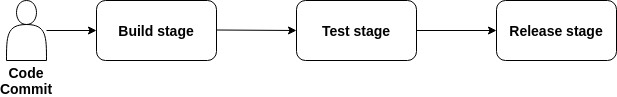
\includegraphics[width=14cm]{figures/pipeline.png}
    \captionsetup{justification=centering,margin=2cm}
    \caption{A simple example CI pipeline, consisting of a few stages, starting with a developer uploading a change of code}
    \label{fig:pipeline}
\end{figure}

Each stage of a pipeline may be either passed or failed. The failed stage indicates that some particular code change cannot satisfy the requirements of that particular stage. The stages are run in a specific order. In figure ~\ref{fig:pipeline}, the order is demonstrated with arrows. The first stage is build, then test, then release. Should the build stage fail, then neither the test nor the release stage will be run.

There exists an extension of continuous integration and it is called: \textbf{Continuous delivery (CD)}. CD verifies that a piece of software is always in a deployable state. CD is thus even more attractive than CI, because it offers even more automation \cite{online-do-cicd}.

\subsubsection{Infrastructure as Code}
Together with automation and DevOps there comes the term: \textbf{Infrastructure as Code (IaC)}. IaC may be understood as an approach to automate the infrastructure based on practices from software development. Consistent and repeatable routines are encouraged for infrastructure provisioning and configuration. There are three core practices required to implement IaC: \textbf{define everything as code} (e.g. the configuration can be saved as YAML files), \textbf{continuously validate the code} and, \textbf{build a system from small, loosely-coupled pieces} \cite{book-iac}.

Back in time, developers dealt with software, while operations teams worked on hardware and the operating systems. Now, the hardware is in the cloud and thus, it can be handled in the same way as software. \textbf{The DevOps movement brings software development skills to operations}. It concerns both: tools and workflows \cite{book-cndwk}. The movement from deployment on-premises to the cloud also deserves a few words, but it will be handled in the subchapter: \ref{section-aws}.

\subsection{AWS - The Amazon Cloud} \label{section-aws}
\textit{This subchapter offers an introduction to cloud computing and AWS cloud and also the explanation why this particular cloud was chosen.}
\\

There are three revolutions going on \cite{book-cndwk}:
\begin{itemize}
\item the creation of the cloud,
\item the dawn of DevOps,
\item coming of containers.
\end{itemize}

These revolutions are interlinked and happen all at once. This subchapter focuses on the cloud revolution. The days of "bare-metal", before cloud, are referred to as \textbf{"Iron Age"} \cite{book-cndwk,book-iac}. The current times (after cloud was invented) are called \textbf{"Cloud Age"} and the cloud infrastructure - \textbf{Infrastructure as a Service (IaaS)}. IaaS allows to outsource not only the hardware but also the software. The outsourced software involves: operating systems, networking scripts, monitoring logic etc. \textbf{Managed services} can take care of many non-functional requirements. There is no more grand upfront investment. Having a large-scale system to build may have cost a fortune in the past. Back then, the computing power was a capital expense and now --- it is an operational one. Now, there is no fixed cost and the expense depends most often on cloud resources utilization \cite{book-cndwk, article-aws-architecting}.

\textbf{Cloud computing} may be defined as a model that provides end users with access from any device, as long as the device has an Internet access, to a shared set of cloud resources. The cloud resources involve various servers and services. Taking a step away, there may be differentiated four \textbf{deployment models}: private cloud, community cloud, public cloud, hybrid cloud. Private cloud means that the software is deployed on-premises, locally. Apart from that, there are also \textbf{service models}, which the most popular are \cite{article-poni-cloud}:
\begin{itemize}
\item Infrastructure as a Service (IaaS),
\item Platform as a Service (Paas),
\item Software as a Service (Saas).
\end{itemize}

Public clouds like: Amazon AWS, Google Cloud Platform or Microsoft Azure represent IaaS. In the Amazon whitepaper "Architecting for the Cloud" \cite{article-aws-architecting}, many \textbf{cloud computing benefits} are listed:
\begin{itemize}
\item near zero upfront infrastructure investment,
\item just-in-time infrastructure --- meaning that it is simple to scale the applications,
\item more efficient resource utilization --- resources can be reserved or required on demand (instantly),
\item usage-based costing --- users do not pay for allocated but unused infrastructure,
\item reduced time to market --- some jobs can be run parallely.
\end{itemize}

Furthermore, AWS offers \textbf{a highly reliable and scalable infrastructure} \cite{article-aws-architecting}, ensures \textbf{attractive SLAs} (e.g. AWS promises to keep a Monthly Uptime Percentage of at least 99.99\% for compute resources) \cite{online-aws-sla} and it is also \textbf{widely adopted and provides many various services} \cite{cncf-2019}. These are the reasons why AWS was chosen for this thesis. The charts in figures \ref{fig:cncf-aws-pop1} and \ref{fig:cncf-aws-pop2} present the popularity of AWS solutions.

\begin{figure}[H]
    \centering
    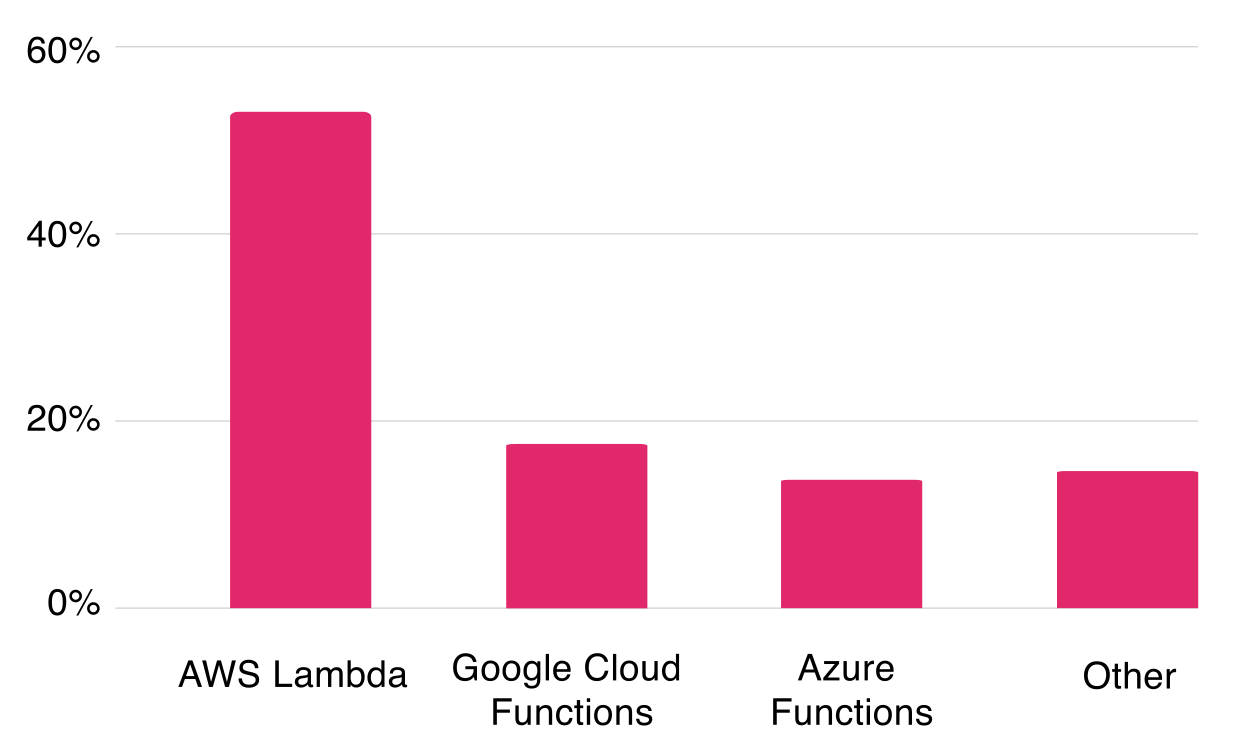
\includegraphics[width=8cm]{figures/cncf-aws-pop1.png}
    \captionsetup{justification=centering,margin=2cm}
    \caption{Hosted serverless platforms preferred by CNCF community during September and October 2019 \cite{cncf-2019}}
    \label{fig:cncf-aws-pop1}
\end{figure}
\begin{figure}[H]
    \centering
    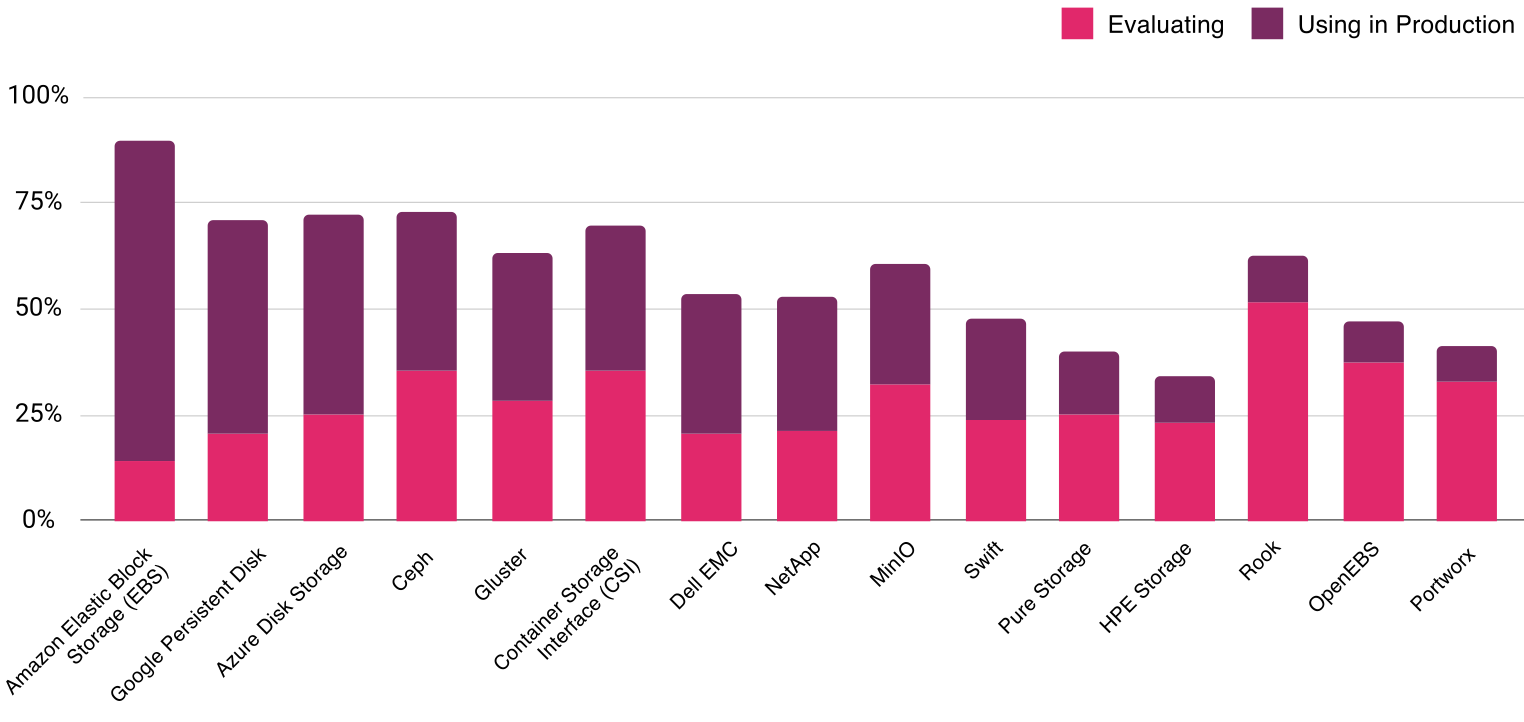
\includegraphics[width=13cm]{figures/cncf-aws-pop2.png}
    \captionsetup{justification=centering,margin=2cm}
    \caption{Cloud native storage preferred by CNCF community during September and October 2019 \cite{cncf-2019}}
    \label{fig:cncf-aws-pop2}
\end{figure}

\textbf{CNCF} is an abbreviation from \textit{Cloud Native Computing Foundation}. It is a non profit organization which fosters communities to support growth and health of cloud native open source software. CNCF adopts Cloud Native projects and catalogs them, depending on their maturity level. They also regularly conduct surveys concerning the Cloud Native and container-related technologies \cite{cncf-services}.



\subsection{Docker containers}
\textit{This subchapter provides an introduction to Docker containers and also compares them to Virtual Machines.}

In the old times, software was installed \textbf{on physical hardware directly}. Then, \textbf{virtualization and Virtual Machines (VMs)} were invented. The next great invention, after VMs, were \textbf{Docker containers}. In 2013 Docker was created as a standard way to manage containers\cite{book-devops-k8s}.

There are many advantages of using VMs and Docker containers in comparison to physical hardware. Docker containers and VMs:
\begin{itemize}
\item provide safer, isolated environment --- facilitate experiments,
\item are easier to automate, manage and replace,
\item provide reproducible environment,
\item limit "works on my machine" problem,
\item offer more security, e.g. an external user may have access only to a Docker container, not to a whole physical host,
\item have additional features, e.g. memory replication.
\end{itemize}

It is claimed, that containers may be replacing VMs. One reason for this might be that there is a significantly lower overhead in case of deploying containers compared to VMs \cite{article-modelling-performance-k8s}. Furthermore, in comparison to VMs, containers provide faster resource allocation. There are many implementation of containers, but among them, Docker is probably the most adopted \cite{article-state-machine}.

Docker uses some major Linux kernel features like: \textbf{namespaces and cgroups}. Namespaces control and limit the amount of resources a process can use, while cgroups manage the resources of a process group. They both help to provide isolation and resource limitation \cite{art-byza,book-devops-k8s}.

In order to be able to work with Docker containers, one has to know the \textbf{difference between a Docker container and a Docker image}. A Docker image is a read-only template. It has some software installed and configured. Each image has a name and a tag, which serves the same purpose as a software version. One image may be based on other image. There are many images available which are open-source and free, e.g. "debian:10.3" \cite{online-dh-debian}, "ubuntu:16.04" \cite{online-dh-ubuntu}. It is easy to build one’s own image, basing on the available images \cite{online-docker-doc}.

Below, there is an example of a source code which creates (builds) a Docker image. Just one file is enough for this task: \textbf{a Dockerfile} (listing \ref{lst:dockerfile}).

\begin{lstlisting}[basicstyle=\small,caption={A Dockerfile to build a Docker image with SSH server installed. Based on Docker official documentation \cite{online-docker-doc-bi}},captionpos=b,language=Bash,xleftmargin=0.3cm,label={lst:dockerfile}]
FROM ubuntu:16.04

RUN apt-get update && apt-get install -y openssh-server
RUN mkdir /var/run/sshd
RUN echo 'root:THEPASSWORDYOUCREATED' | chpasswd
RUN sed -i 's/PermitRootLogin prohibit-password/PermitRootLogin\
  yes/' /etc/ssh/sshd_config

# SSH login fix. Otherwise user is kicked off after login
RUN sed 's@session\s*required\s*pam_loginuid.so@session\
  optional pam_loginuid.so@g' -i /etc/pam.d/sshd

ENV NOTVISIBLE "in users profile"
RUN echo "export VISIBLE=now" >> /etc/profile

EXPOSE 22
CMD ["/usr/sbin/sshd", "-D"]
\end{lstlisting}

Docker containers are claimed to be \textbf{lightweight and portable}. Thus, containers are suitable for microservices. Since microservices are loosely-coupled, failure of one microservice should not affect other microservices of an application. This architectural style is characterized by fine granularity and therefore, it makes scaling more flexible and efficient \cite{article-k8s-as-avail}.

Docker containers are utilized by big companies like:  \textbf{Netflix or Twitter} \cite{article-nonf-twitter-netflix}. Docker is a technology described thoroughly in many literature sources and therefore there is no sense in repeating it. A curious reader is referred to read the official Docker documentation \cite{online-docker-doc}.

\subsection{Kubernetes as a Docker containers orchestration system}
\textit{This subchapter describes what Kubernetes is and what problems it solves. Furthermore, the chapter acknowledges Kubernetes popularity and briefly introduces chosen Kubernetes objects.}
~\\
~\\
The process of deploying multiple containers of one application can be optimized through automation. This kind of automation is referred to as \textbf{orchestration} \cite{art-byza}.

There was a need to automatically deploy and manage a large number of services at global scale on millions of servers. Thus, Google developed Borg. Borg is a private orchestration system. It is very powerful, but also very much coupled to Google’s own internal and proprietary technologies. Therefore, in 2014 Google launched a new project called: \textbf{Kubernetes}. The name comes from a Greek word which means "helmsman, pilot". Apart from Kubernetes, there are alternative solutions invented, other orchestrators, but Kubernetes \textbf{won the orchestration wars} \cite{book-cndwk,article-modelling-performance-k8s}.

"Kubernetes does the things that the very best system administrator would do: automation, failover, centralized logging, monitoring. It takes what we’ve learned in the DevOps community and makes it the default, out of the box." These are the words uttered by Kelsey Hightower --- a Google employee with legendary contributions to Kubernetes \cite{book-cndwk}.

Kubernetes was built \textbf{to make deployments easy, to reduce the time and effort} which needs to be poured into them. To achieve this goals, Kubernetes offers \textbf{a wide variety of features}\cite{k8s,book-cndwk,article-state-machine}:
\begin{itemize}
\item creating, destroying, replicating containers,
\item rolling updates of containers,
\item built-in health checks (liveness and readiness probes),
\item autoscaling,
\item redundancy and failover --- to make the applications deployed on top of Kubernetes more resilient and reliable,
\item being provider-agnostic --- Kubernetes can be deployed on-premises and in the cloud and in both cases it will provide the same set of features, thus, it may be said that Kubernetes unifies the underlying infrastructure,
\item utilizing provider-specific (sometimes referred to as: vendor-specific) features, e.g. AWS load balancer or Google Cloud load balancer,
\item self-healing,
\item service discovery,
\item load balancing,
\item storage orchestration.
\end{itemize}


Kubernetes is the first project of the CNCF \cite{article-state-machine}. Kubernetes is already \textbf{used by some well-known entities}, e.g. NASA \cite{nasa}, F-16 jets \cite{online-f16}, Zalando \cite{online-zalando}, ING \cite{online-ing}, booking.com \cite{online-bookingcom}. Apart from that, the \textbf{Kubernetes popularity is growing}, basing on the information from CNCF Survey 2019, which states that 78\% of respondents use Kubernetes in production and that this is a huge jump from 58\% using in the previous --- 2018 year \cite{cncf-2019}. Even the older CNCF Survey from year 2017 shows Kubernetes as number one cloud management platform --- it it presented in figure \ref{fig:cncf-con}.

The \textbf{basic working unit in Kubernetes is a pod}. A pod is an abstraction and it represents one application, a set of containers. Two things are crucial to know about pods \cite{article-modelling-performance-k8s}:
\begin{itemize}
\item all the containers defined in a pod will be deployed on one machine,
\item a pod has one IP address assigned and all the containers defined in this pod share the same IP address.
\end{itemize}

A pod is all that is needed to deploy a set of containers. Pod is a Kubernetes object and there are many more objects, for example: deployment, replica sets, service, ingress. The important thing to note is that these \textbf{objects can be configured in a declarative way}, thanks to \textit{YAML} files \cite{k8s-declarative}.

Kubernetes provides mechanisms for maintaining, deploying, healing and scaling containerized microservices. Thanks to that, Kubernetes hides the complexity of microservices orchestration. It is much easier to satisfy non-functional requirements of microservices deployment by using Kubernetes. An example of such requirements may be: availability, healing, redundancy or autoscaling \cite{article-k8s-as-avail}.

\begin{figure}[H]
    \centering
    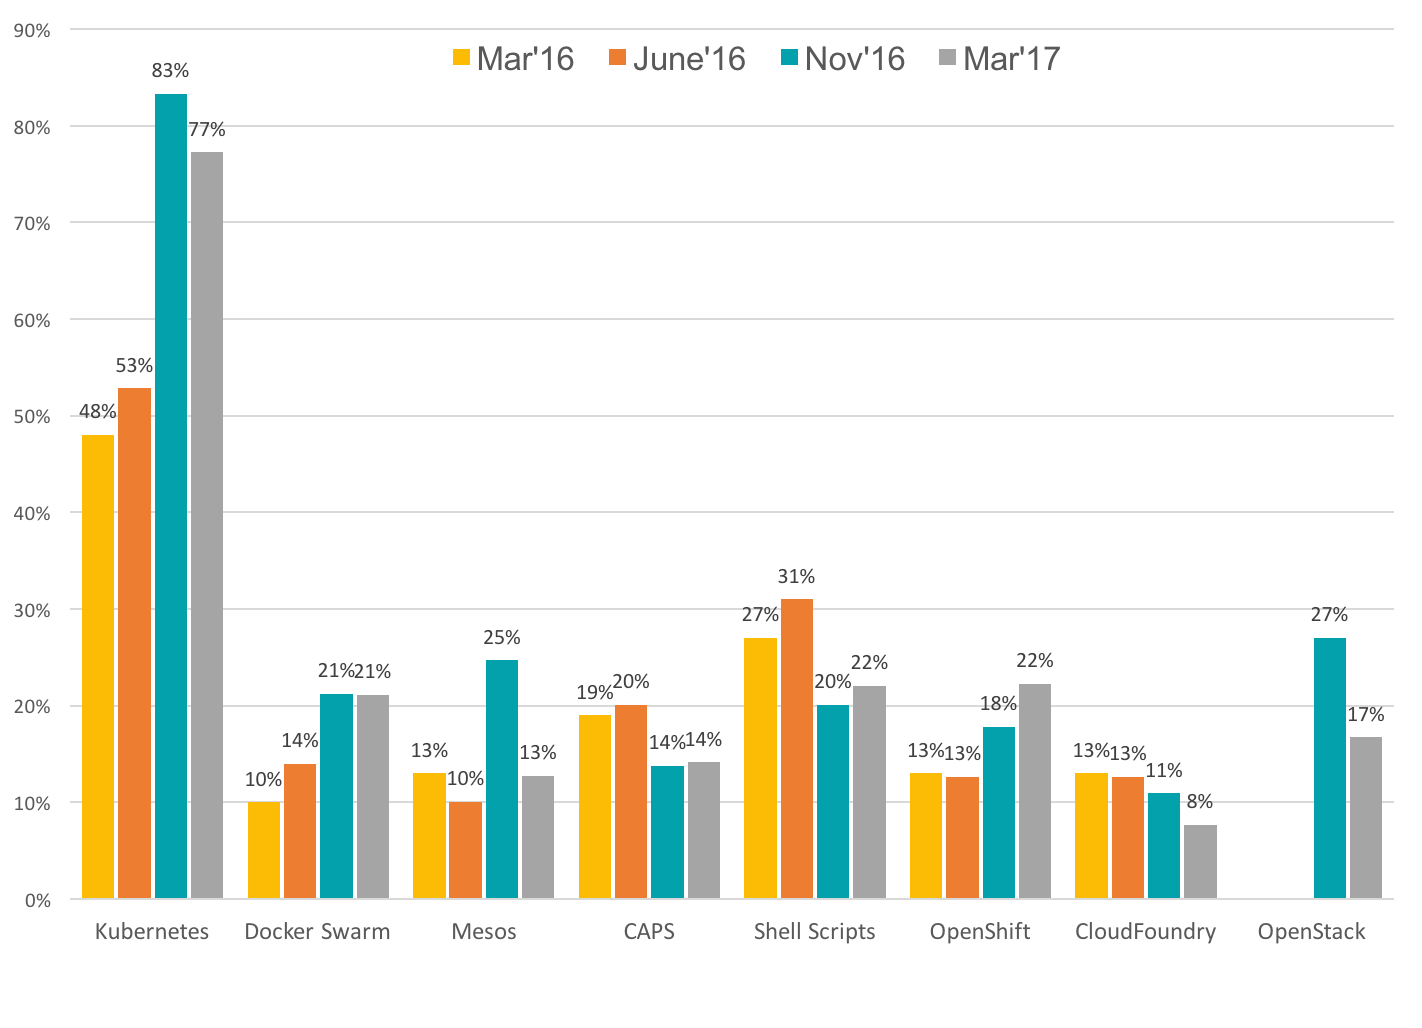
\includegraphics[width=14cm]{figures/cncf-container-orchestrators.png}
    \captionsetup{justification=centering,margin=2cm}
    \caption{Results of CNCF Survey from year 2017 showing Kubernetes as number one cloud management platform \cite{cncf-2017}}
    \label{fig:cncf-con}
\end{figure}



\subsection{Kubernetes architecture}
% this short summary before each subchapter helps me to stay focused on what i want to write about
\textit{This subchapter contains a high level description of the Kubernetes architecture. The focus is on the responsibilities of each Kubernetes component.}

\subsubsection{Kubernetes cluster}
A \textbf{Kubernetes cluster} may be defined as a collection of storage and networking resources which are used by Kubernetes to run various workloads \cite{book-mastering-k8s}. Another definition states that a Kubernetes cluster is a single unit of computers which are connected to work together and which are provisioned with Kubernetes components \cite{k8s-cluster}.

A cluster consists of two kinds of instances: masters and nodes. An instance can be a virtual machine or a physical computer \cite{article-k8s-as-avail,k8s-cluster}. This is depicted in figure ~\ref{fig:cluster-k8s}. Kubernetes nodes communicate with Kubernetes master.
\begin{figure}[H]
    \centering
    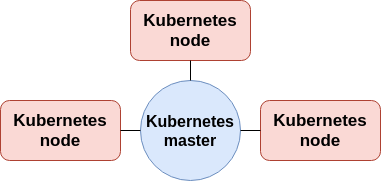
\includegraphics[width=10cm]{figures/cluster-k8s.png}
    \caption{Kubernetes cluster diagram depicting a master-slave architecture}
    \label{fig:cluster-k8s}
\end{figure}

\subsubsection{Masters and nodes}
\textbf{The role of the master is to manage the cluster}. This means that master: schedules applications, maintains their desired state, scales them, handles events, manages nodes. \textbf{Nodes serve as the worker machines}. They are responsible for running containers and handling container operations. Masters schedule containers to run on nodes \cite{book-mastering-k8s, k8s-cluster}. At least one node and one master is needed in a Kubernetes cluster. In order to provide fault-tolerance and high availability in production environments, multiple master and multiple node instances are run \cite{k8s-components}.

The instances in a Kubernetes cluster (masters and nodes) are hosts to several \textbf{Kubernetes components}. There are \textbf{master components}, used to control the cluster and there are also \textbf{node components}, run on each node. All the components are presented in figure \ref{fig:components-of-kubernetes}:
\begin{figure}[H]
    \centering
    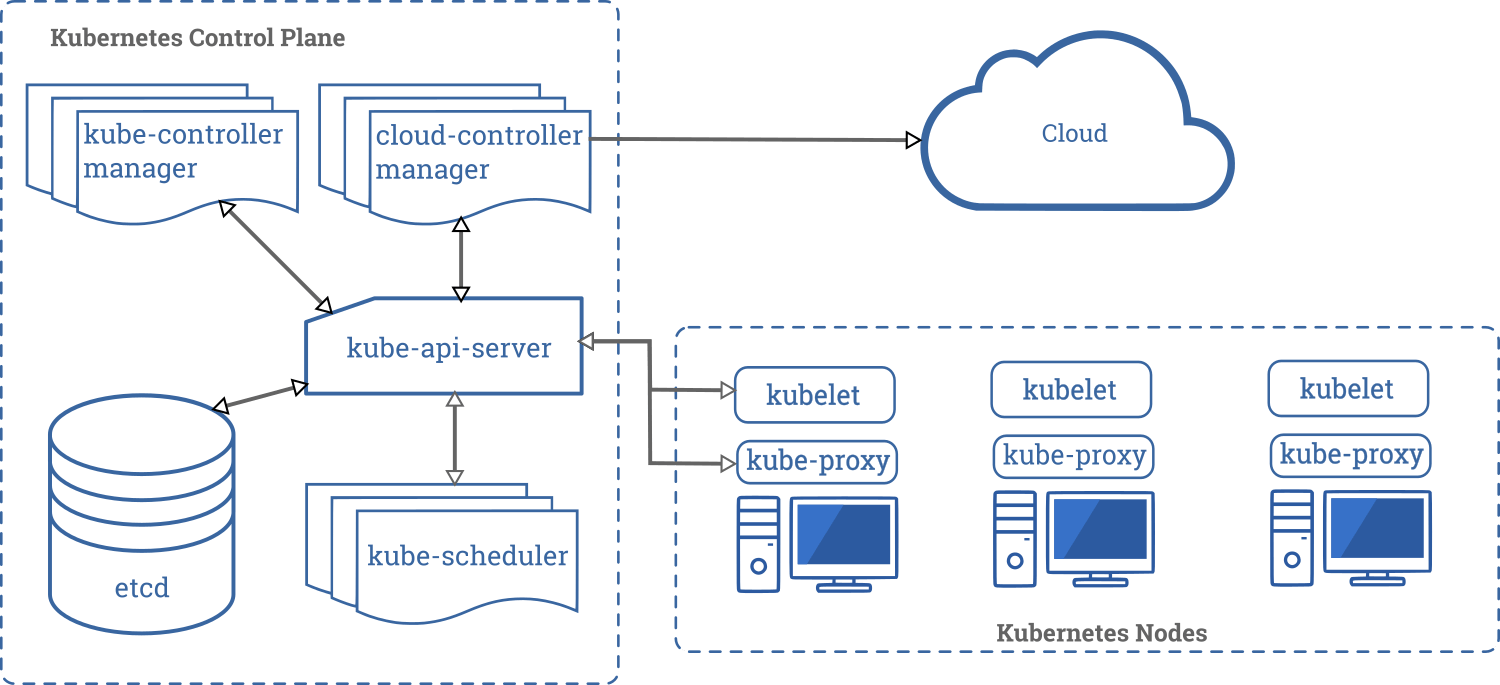
\includegraphics[width=14cm]{figures/components-of-kubernetes.png}
    \caption{Kubernetes components including master and node components \cite{k8s-components}}
    \label{fig:components-of-kubernetes}
\end{figure}


\subsubsection{Components}
The master components are also known as the control plane’s components. They are as follows \cite{book-mastering-k8s, k8s-components}:
\begin{itemize}
\item Etcd (a key-value store),
\item API server,
\item Scheduler,
\item Controller manager and Cloud Controller manager.
\end{itemize}

\paragraph{}
\textbf{Etcd} stores the entire cluster state. It is a highly-available key-value store. It is enough, for a test Kubernetes cluster, to deploy one instance of Etcd. However, for the purposes of high availability and redundancy, a 3-node or even 5-node Etcd cluster is typical. It is recommended to have a back up plan for the data stored in Etcd\cite{book-mastering-k8s,k8s-components}. The name \textit{etcd} follows a naming convention within the UNIX directory structure. In UNIX, all system configuration files are contained in a folder called "/etc". The last letter "d" stands for "distributed" \cite{etcd-name}.

\textbf{API server} exposes the Kubernetes REST API. It allows the nodes to communicate with the master and it also allows end users to interact with the cluster. Thanks to the fact that API server is stateless and that all its data is stored in etcd, API server can easily scale horizontally. The main implementation of a Kubernetes API server is kube-apiserver\cite{book-mastering-k8s,k8s-components,k8s-cluster}.


\textbf{Scheduler} is responsible for assiging containers to nodes. Scheduler selects a node for a container to run on. It considers a range of factors: resource requirements, various constraints, affinity and anti-affinity specifications, data locality, inter-workload interference, and deadlines. The implementation is known as kube-scheduler \cite{book-mastering-k8s, k8s-components}.

\textbf{Controller manager} runs controller processes such as: watching the shared state of the cluster and making changes needed to move the current state into the desired state. Controller manager is a collection of separate managers, but they are all compiled into a single binary and run in a single process in order to reduce complexity. The controllers consist of: Node Controller, Replication Controller, Endpoints Controller, Service Account and Token Controllers. The implementation of Controller manager is kube-controller-manager \cite{book-mastering-k8s, k8s-components}.

\textbf{Cloud Controller manager} interacts with a specified underlying cloud provider (e.g. Amazon Web Services or Google Cloud Platform). It is implemented by cloud-controller-manager and therefore, it allows the Kubernetes code and the cloud vendor’s code to evolve independently \cite{k8s-components}.

As aforementioned, there are also node components. They run on both: masters and nodes. They are as follows \cite{book-mastering-k8s, k8s-components}:
\begin{itemize}
\item Kubelet,
\item Proxy,
\item Container Runtime.
\end{itemize}

\textbf{Kubelet} oversees the communication with the master components (by monitoring API server for changes) and makes sure that containers, described by a Pod, are running and healthy (so it manages a Pod lifecycle). A Pod is a simple object from a Kubernetes API and it represents a set of containers. Containers which were not created by Kubenernetes are not managed by Kubelet \cite{book-mastering-k8s, k8s-components}.

\textbf{Proxy} is implemented by kube-proxy. It is a network proxy and it implements a part of the Kubernetes Service concept, which means that it is responsible for exposing an application as a network service and it provides load balancing \cite{book-mastering-k8s, k8s-components}.

\textbf{Container Runtime} is the software which is responsible for operating containers. Several container runtimes are supported: Docker, containerd, CRI-O, and any implementation of the Kubernetes CRI (Container Runtime Interface). It is a design policy of Kubernetes that is ought to be decoupled from a specific container runtime. Under some circumstates it should be possible to switch from one container runtime to another or to use multiple of them at once. Originally, Kubernetes was designed to manage only Docker containers \cite{book-mastering-k8s, k8s-components}.

\subsubsection{Other services}
\label{k8s-other-services}
Apart from master and node components, there are also \textbf{add-ons, extensions, and third party tools} which communicate with Kubernetes by the API server and which provide additional functionality. Examples of such services are: DNS, Vertical Pod Autoscaler, Cluster Autoscaler, Istio, Kubernetes Dashboard, kube-ops-view, node-problem-detector, etc \cite{book-cndwk}}.

\subsubsection{The Kubernetes networking model}
\label{k8s-net}
Kubernetes states a few \textbf{networking requirements} \cite{k8s-net}:
\begin{itemize}
\item pods on a node must be able to communicate with all pods on all nodes without Network Address Translation (NAT),
\item agents on a node (e.g. system daemons, kubelet) must be able to communicate with all pods on that node.
\end{itemize}

There are many available options that help with satisfying these requirements, e.g. AWS VPC CNI for Kubernetes, Azure CNI for Kubernetes, Flannel, OpenVSwitch, Project Calico, etc \cite{k8s-net}. CNI stands for Container Networking Interface and it is a specification and also a set of libraries for writing network plugins to configure network interfaces in Linux containers. A CNI container is bound to have its own IP address. For Kubernetes, \textbf{each pod has its own IP address}, so the pod is the CNI container \cite{book-mastering-k8s}. \textbf{Containers that belong to a one pod share the same IP address}, which means that these containers can reach all reach each other’s ports on localhost and also that none two containers should expose the same port. This model is known as "IP-per-pod" \cite{k8s-net}.

\subsection{Production deployment requirements}
\textit{This section explains what a production deployment is and what requirements it must met.}
~\\

\subsubsection{Multiple environments in software deployment}
First, it is helpful to distinguish between the terms: \textbf{'infrastructure stack' and 'environment'}. They both may be defined as a collection of infrastructure resources. The difference is that \textbf{an environment is conceptual, while a stack is concrete}. A stack is defined with code, particularly when Infrastructure as Code is applied, and managed using tools. However, an environment serves to fulfill a predetermined purpose. Multiple environments can run an instance of the same system\cite{book-iac}.

Typically, there are \textbf{two reasons for which multiple environments are in use}: to support a release delivery process and to run multiple production instances of the system. The first reason allows to have a particular build of an application (e.g. a git commit or a specified version of code) well tested. Such a build has to go through many different environments, e.g.: testing, staging and production. When a build does not pass all the stages in the former environments, it will not be promoted to the production environment\cite{book-iac}\cite{book-cicd}.

To briefly explain the second reason for multiple environments: they are used in order to ensure fault-tolerance (when one environment fails, the other can take over), scalability (the work can be spread among many clusters), segregation (it may be decided to handle a group of customers using one environment and the other group with the other environment, e.g. for latency purposes)\cite{book-iac}. Well-known examples of running multiple production deployments can be \textbf{Blue-green deployments or Canary deployments}\cite{bachelor-ha}.

\subsubsection{Production deployment requirements}
\label{Production deployment requirements}
Throughout this work a production deployment means such a deployment which targets the production environment. A list of \textbf{requirements for a production deployment}, gathered through the literature, is provided below:
\begin{itemize}
\item \textbf{Central Monitoring} - this is helpful when troubleshooting a cluster\cite{book-mastering-k8s}\cite{online-weave-checklists}\cite{online-weave-guide}\cite{book-cndwk}.
\item \textbf{Central Logging} - this is a fundamental requirement for any cluster with number of nodes or pods or containers greater than a couple\cite{book-mastering-k8s}\cite{online-weave-checklists}\cite{book-devops-k8s}.
\item \textbf{Audit} - to show who was responsible for what action\cite{online-weave-guide}.
\item \textbf{High Availability} - authors of \cite{book-mastering-k8s} go even further and state that the cluster should be tested for being reliable and highly available \textbf{before} it is deployed into production\cite{book-mastering-k8s}\cite{book-cndwk}.
\item \textbf{Live cluster upgrades} - it is not affordable for large Kubernetes clusters with many users to be offline for maintenance\\cite{book-mastering-k8s}.
\item \textbf{Backup, Distaster Recovery}\cite{book-mastering-k8s}\cite{online-weave-guide}\cite{book-cndwk}.
\item \textbf{Security, secrets management, image scanning} - security at many levels is needed (node, image, pod and container, etc.)\cite{book-mastering-k8s}\cite{online-weave-checklists}\cite{online-weave-guide}\cite{book-cndwk}.
\item \textbf{Passing tests, a healthy cluster} - 'if you don't test it, assume it doesn't work'\cite{book-mastering-k8s}\cite{book-cndwk}.
\item \textbf{Automation and Infrastructure as Code} - in production environment a versioned, auditable, and repeatable way to manage the infrastructure is needed\cite{book-mastering-k8s}\cite{online-weave-guide}.
\item \textbf{Autoscaling} - if application deployed on a Kubernetes demand more resources, then a new Kubernetes node should be automatically created and added to the cluster. However, autoscaling, even though nice to have, is not that important\cite{book-cndwk}.
\end{itemize}

\subsubsection{Monitoring as production environment requirement}
\textbf{Monitoring} helps to ensure that a cluster is operational, correctly configured and that there are enough resources deployed. Monitoring is also indispensable for debugging and troubleshooting\cite{book-mastering-k8s}. The third reason for using a monitoring system is that historical data is needed for planning purposes. The monitoring strategy should cover four areas\cite{book-cicd}:
\begin{itemize}
\item configuring the infrastructure in such a way that it is possible to collect the data,
\item storing the data,
\item providing dashboards, so that data is presented in a clear way,
\item setting up notifications or alarms to let people know about certain events.
\end{itemize}
\paragraph{}
Monitoring provides various \textbf{metrics}, e.g.: CPU usage, memory utilization, I/O per disk, disk space, number of network connections, response time, etc. Thus, it is helpful on many different levels: on hardware, operating system,  middleware and application level. There is a wide range of \textbf{available open source and commercial tools} to take care of monitoring: Nagios, OpenNMS, Flapjack, Zenoss, Tivoli from IBM, Operations Manager from HP, Splunk, etc.\cite{book-cicd}. Solutions recommended for a Kubernetes cluster are: Heapster combined with InfluxDB as backend and Grafana as frontend and also cAdvisor\cite{book-mastering-k8s}. A nice feature of Grafana are its dashboards. Example Grafana dashboard is presented in the next image:
\begin{figure}[H]
  \centering
  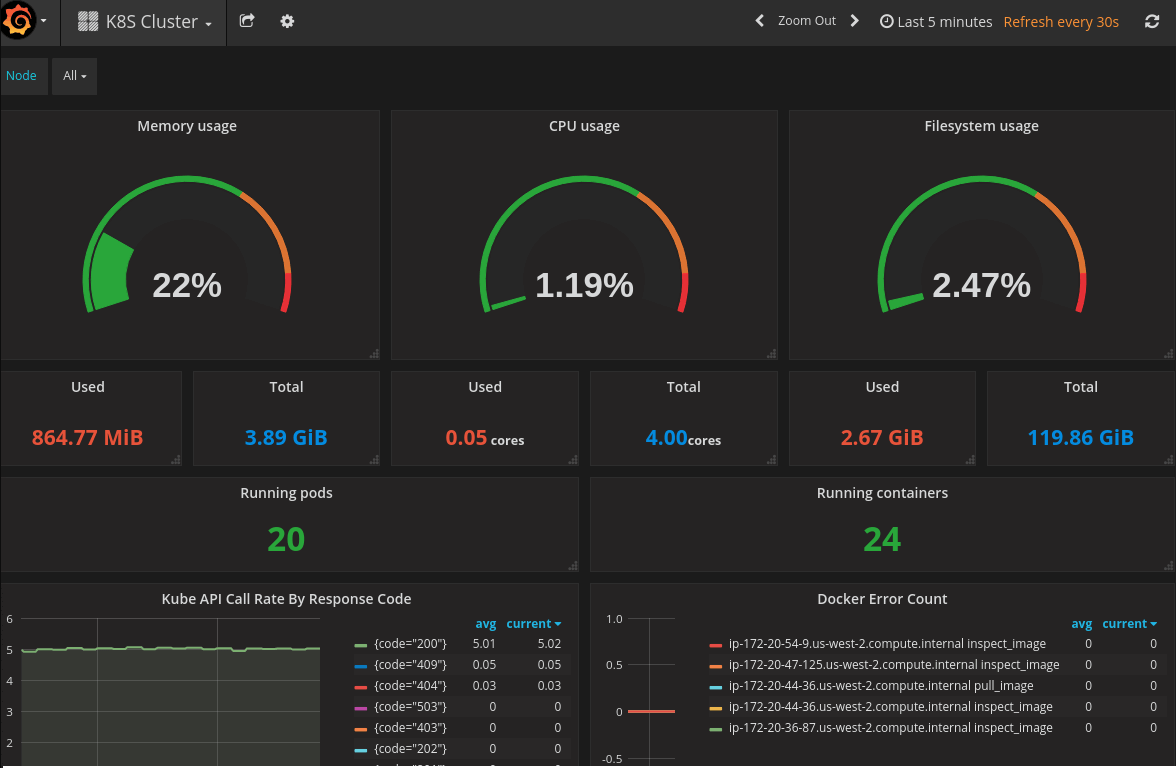
\includegraphics[width=11cm]{figures/grafana.png}
  \label{fig:grafana}
  \caption{Example Grafana dashboard for a Kubernetes cluster, showing among others: Memory, CPU and File system usage\cite{monitor-kubernetes-cluster-prometheus-grafana}}
\end{figure}
Grafana also works well with Prometheus, which is a monitoring system and a time series database. Prometheus is also a CNCF graduated project\cite{online-prometheus-gh}\cite{online-prometheus-www}. If a system (like Kubernetes) is deployed on AWS, another solution for monitoring and logging may be: Amazon CloudWatch\cite{online-cw}.

Another solution for monitoring is Kubernetes dashboard, which is a built-in solution and doesn't require any customization. Heapster, InfluxDB and Grafana are great for heavy-duty purposes, whereas Kubernetes dashboard is probably able to satisfy the majority of monitoring needs of a Kubernetes cluster\cite{book-mastering-k8s}\cite{book-devops-k8s}. Example dashboard provided by Kubernetes dashboard is depicted on the next image:
\begin{figure}[H]
  \centering
  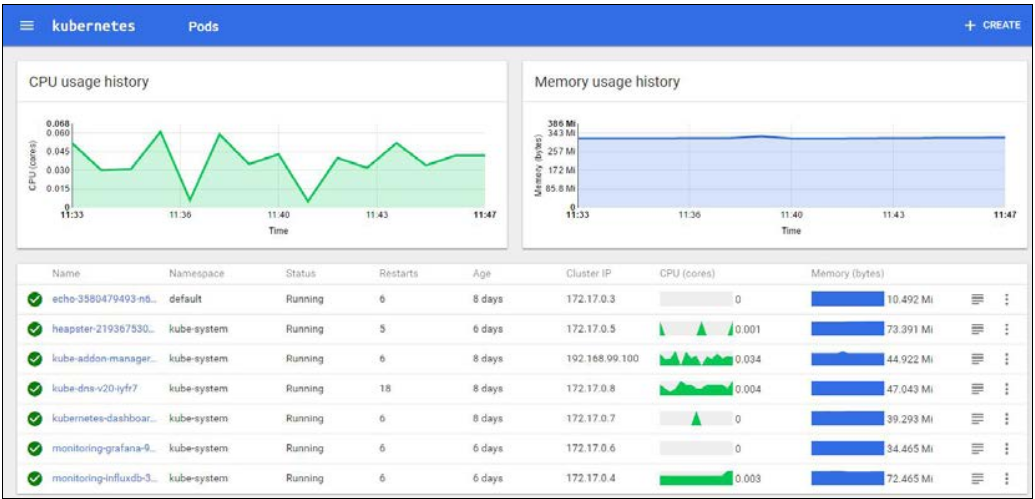
\includegraphics[width=10cm]{figures/k8s-dashboard.png}
  \caption{Kubernetes dashboard depicting CPU and Memory usage by Kubernetes pods\cite{book-mastering-k8s}}
\end{figure}

\subsubsection{Logging as production environment requirement}
Kubernetes dashboard has also a feature which makes it able to show \textbf{log messages} of a single container deployed on Kubernetes\cite{book-mastering-k8s}. \textbf{Centralized logging} is essential for a production cluster, because usually there are a lot of pods (and containers) deployed, each generating many log messages. It is impossible to require a Kubernetes administrator to login into each container for the purpose of getting the logs.

The second reason for the importance of centralized logging is that \textbf{containers are ephemeral} - the log messages kept inside the containers would be lost after a container is redeployed. \textbf{Popular solutions} are: Fluentd, Elasticsearch, Kibana\cite{book-mastering-k8s}, Logstash\cite{book-devops-k8s} and Graylog\cite{online-prod-year-k8s}\cite{online-graylog}. It is also important to consider that log messages in Kubernetes cluster are generated from many sources: from end-user applications, nodes, Kubernetes system containers and there are also \textbf{audit logs} in the form of e.g. api server events\cite{online-graylog-art}. For the purposes of auditing, when deploying on AWS, one can use AWS CloudTrail\cite{online-ct}.

\subsubsection{High Availability as production environment requirement}
While administering a Kubernetes cluster, there is a high probability that something will go wrong. Components, network can fail, configuration can be incorrect, people make mistakes and software has bugs. Failure classification has been described in \cite{article-failures}. This has to be accepted and a system should be designed in such a way that it is \textbf{reliable and highly available (HA)} despite of many problems. Here is a list of ideas how to ensure high availability\cite{book-mastering-k8s}:
\begin{itemize}
\item \textbf{Redundancy} - means having a spare copy of something. Kubernetes uses Replica Sets or Replication Controllers to provide redundancy for applications deployed on Kubernetes. Five redundancy models were summarized in \cite{article-redundancy-models}. Some of them require an active replica (running) and other passive (or standby).
\item \textbf{Hot Swapping} - can be explained as replacing some failed component on the fly, with minimal or ideally zero down-time. Actually, hot swapping is quite easy to implement for stateless applications. For stateful applications, one has to keep a replica of a component (see redundancy).
\item \textbf{Leader election} - it is a pattern used in distributed systems. Whenever there are many servers fulfilling the same purpose to share the load. One of the servers must be elected a leader then and certain operations must go through it. When the leader server experiences a failure, other server can be selected as new leader. This is a combination of redundancy and hot swapping.
\item \textbf{Smart load balancing} - used to share and distribute the load.
\item \textbf{Idempotency} - means that one request (or some operation) is handled exactly once.
\item \textbf{Self-healing} - means that whenever a failure of one component happens, it is automatically detected and steps are taken (also automatically) to get rid of the failure.
\item \textbf{Deploying in a cloud} - a goal is to be able to physically remove or replace a piece of hardware, either because of some issues or because of preventative maintenance or horizontal growth. Often this is too expensive or even impossible to achieve\cite{article-failures}. Traditional deployments on-premises forced administrators to do a capacity planning (to predict the amount of computing resources). Thanks to the on-demand and elastic nature of the clouds, the infrastructure can be closely aligned to the actual demand. It is also easy to scale applications deployed on a cloud, because of the fundamental property of the cloud: elasticity\cite{article-aws-architecting}.
\end{itemize}

Generally speaking, \textbf{"highly available systems are fault tolerant systems with no single point of failure"}\cite{article-redundancy-models}. In order to introduce HA for the Kubernetes cluster the following ideas could be incorporated\cite{book-mastering-k8s}:
\begin{itemize}
\item Deploy Etcd as a cluster, not just one instance of Etcd.
\item Ensure redundancy for api server.
\item Deploy multiple master instances and ensure a load balancer in front of them.
\item Ensure that node instances are reliable: the Docker daemon and the Kubelet daemon should restart automatically in case of failure.
\item Apply RAID to ensure redundancy of data storage or apply Key-Value Multi-Device (KVMD), a hybrid data reliability manager\cite{data-rel-kv} or let cloud provide storage availability.
\end{itemize}

Furthermore, it may be needed to test high availability. This can be done by inducing a predictable failure and verifying if the system behaves as expected\cite{book-mastering-k8s}. Such a kind of testing, where one or more cluster nodes or pods is killed is called Chaos Monkey, after the tool developed by Netflix. There are also ready to use tools basing on the idea of Chaos Monkey: chaoskube, kube-monkey, PowerfulSeal\cite{book-cndwk}.
\begin{figure}[H]
    \centering
    
\includegraphics[width=3cm]{figures/chaos-monkey-logo.png}
    \label{fig:chaos-monkey-logo}
    \caption{Logo of the Netflix program: Chaos Monkey\cite{chaosmonkey}}
\end{figure}

\subsubsection{Automation as production environment requirements}
\label{Automation as production environment requirements}
When it comes to \textbf{automation}, many guidelines can be found in \cite{book-cicd}. Below are some of them listed:
\begin{itemize}
\item \textbf{Every Change Should Trigger the Feedback Process} - means that every change in code should trigger some pipeline and should be tested (including unit tests, functional acceptance tests, nonfunctional tests). The tests should happen in an environment which is as similar as possible to production. Some tests may run in production environment too\cite{book-cicd}\cite{book-iac}.
\item \textbf{The Feedback Must Be Received as Soon as Possible} - this also involves another rule: fail fast. This guideline suggests that faster tests (or less resource-intensive tests) should run first. If theses tests fail, the code does not get promoted to the next pipeline stages, which ensures optimal use of resources\cite{book-cicd}.
\item \textbf{Automate Almost Everything} - generally, the build process should be automated to such extent where specific human intervention or decision is needed. But there is no need to automate everything at once\cite{book-cicd}\cite{book-iac}.
\item \textbf{Keep Everything in Version Control} - this means that not only application source code but also tests, documentation, database configuration, deployment scripts, etc. should be kept in version control and that it should be possible to identify the relevant version. Furthermore, any person with access to the source code should be able to invoke a single command in order to build and deploy the application to any accessible environment. Apart from that, it should be also clear which version in version control was deployed into each environment\cite{book-cicd}.
\item \textbf{If It Hurts, Do It More Frequently, and Bring the Pain Forward} - if some part of the application lifecycle is painful, it should be done more often, certainly not left to do at the end of the project\cite{book-cicd}.
\item \textbf{Idempotency} - the tools used for automation should be idempotent, which means that no matter how many times the tool is invoked, the result should stay the same\cite{book-iac}.
\end{itemize}

\paragraph{}
Together with automation, there are two inextricably entwined terms: Infrastructure as Code and DevOps. As these two terms has been already explained in this work, now let us focus on the essential tools needed to introduce the automated application lifecycle. First, a framework for \textbf{Configuration Management} is needed. Examples involve: Puppet, CFEngine\cite{book-cicd}\cite{book-iac}, Chef\cite{online-chef}, Ansible\cite{online-ansible}, SaltStack\cite{online-salt}, etc. These tools help to declaratively define what packages should be installed and how should they be configured in a virtual machine or a container or a physical server\cite{book-cicd}. They can help prevent \textbf{configuration drift} in a large number of computers\cite{book-devops-k8s}. A configuration drift is a difference across systems that were once identical. It can be imposed by a manual amendment and also by automation tools which propagated a change only to some of the instances\cite{book-iac}. There are also stack-oriented tools, which follow the same declarative model: Terraform\cite{terraform} and CloudFormation\cite{book-iac}. Another type of needed tools is a building server, examples are: Jenkins, GoCD, Travis - they were already mentioned earlier.

\subsubsection{Security as production environment requirement}
\textbf{Security} is another essential aspect of production deployment and, as mentioned above, it touches many levels. A node breach is a very serious problem and it can happen by someone logging to the instance or having physical access to it. The latter is easily mitigated by not deploying on bare-metal machines but on a cloud instead\cite{book-mastering-k8s}. The former demands some hardening done. There are several ideas that can be implemented for a Kubernetes cluster specifically listed below:
\begin{itemize}
\item ensuring that data is encrypted in transit by using secure api server protocol (HTTPS instead of HTTP)\cite{book-mastering-k8s}.
\item ensuring proper user and permissions management by configuring authentication, authorization, security accounts and admission control in api server \cite{book-mastering-k8s}. When setting up authorization, it is wise to apply \textbf{the principle of least privilege}. This principle recommends that only the needed resources or permissions should be granted\cite{book-cndwk}.
\item utilizing Role-Based Access Control (RBAC) to manage access to a cluster\cite{book-cndwk}.
\item ensuring security keys management and exchange\cite{book-mastering-k8s} by implementing for example automated key rotation.
\item ensuring that used Docker images are neither malicious (deliberately causing some harm) nor vulnerable (allowing some attacker to take control) by keeping them up-to-date and maintaining them instead of using the publicly available ones or by using a private Docker registry\cite{book-mastering-k8s}.
\item using minimal Docker images because the fewer programs there are installed in an image, the fewer potential vulnerabilities there are\cite{book-cndwk}.
\item maintaining a log or audit system\cite{book-mastering-k8s}.
\item utilizing network policies which act in a whitelist fashion and can open certain protocols and ports\cite{book-mastering-k8s}.
\item using secrets. Kubernetes has a resource called: secret, but the problem is, that Kubernetes stores secrets as plaintext in Etcd. This, in turn, means that steps should be taken in order to limit direct access to Etcd\cite{book-mastering-k8s}.
\item prefering managed services, because they will have many security measures already implemented\cite{book-cndwk}.
\item avoid running processes as root user in Docker containers\cite{book-cndwk}.
\item using available programs for security scanning\cite{book-cndwk}.
\end{itemize}

The following illustration presents security features provided by Kubernetes API server:
\begin{figure}[H]
    \centering
    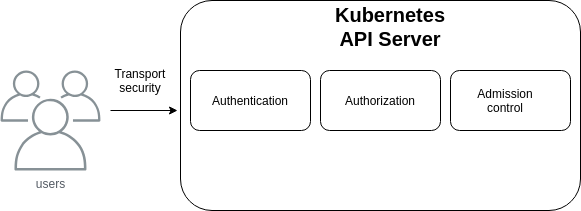
\includegraphics[width=13cm]{figures/api-server-security.png}
    \label{fig:security-api-server}
    \caption{Security features which a request sent to Kubernetes API Server goes through. Based on the official documentation website\cite{k8s-sec}}
\end{figure}

There are many more security measures that Kubernetes administrators and end-users could apply. A curious reader is referred to\cite{book-cndwk} and \cite{book-mastering-k8s}.

\subsubsection{Disaster recovery as production environment requirement}
\textbf{Disaster recovery} can be understood as the process which an organization has to undergo after a service  disruption happened in order to resume normal services. It is vital to know what actions are necessary to overcome the disaster. This set of predefined procedures is known as \textbf{Disaster Recovery Plan}. Furthermore, disaster recovery is not the same as fault tolerance. The latter ensures that a system will withstand and resist the failure\cite{article-dr}.

Disaster recovery is an essential requirement of any business where continuity matters. In order to plan disaster recovery well the following key parameters should be considered: the initial cost, the cost of data transfers and the cost of data storage. Significant costs may be a reason why, in the past, around 40-50\% of small businesses had no DRP and did not intend to change this. However, cloud computing provides affordable solutions, because of the employed model "pay-for-what is used". Another \textbf{advantage of the cloud is that it is fairly easy to use resources deployed in multiple geographical areas}. This is desired, because one the major concepts in a DRP is the geographical separation of the system servers and its backup\cite{article-dr-cloud}.

Key metrics that can be taken into consideration while planning disaster recovery are\cite{article-dr}\cite{article-dr-cloud}:
\begin{itemize}
\item Recovery Point Objective (RPO)
\item Recovery Time Objective (RTO)
\end{itemize}
\textbf{RPO} can be defined as the time between two successive backups. Thus, the time between the last backup and the the disaster, which is de facto the time of data loss, is maximally equal to RPO. \textbf{RTO} can be understood as the time needed to recover from the disaster, when the server experiences downtime\cite{article-dr-cloud}. RPO and RTO are illustrated on the following image:
\begin{figure}[H]
    \centering
    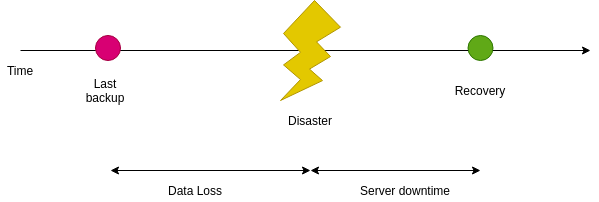
\includegraphics[width=13cm]{figures/rpo-rto.png}
    \label{fig:rpo-rto}
    \caption{RPO and RTO illustrated in relation to time}
\end{figure}

Cloud services mitigate some risks that persistent data storage has. For example: cloud services provide high-available data storage by replicating it across different geographical locations. However, replication is not the same as backup and it does not protect against accidentally deleting a volume or against a misconfigured application overwriting the data. Thus, backup is still needed. In order to backup Kubernetes, the Etcd database has to be backuped. Apart from that, each application deployed on top of Kubernetes should be backuped on its own\cite{book-cndwk}. There are already available services that help with Kubernetes backup: Velero\cite{book-cndwk}.

\subsubsection{Testing as production environment requirement}
Before the production Kubernetes cluster is ready for end-users, it must be verified that \textbf{it works and is healthy}. Every component and every node should be tested proving that it is working as expected. Sometimes, applications expose a custom \textbf{health endpoint}\cite{book-devops-k8s}. E.g. kube-scheduler does that. Thanks to that, it is possible to verify regularly that a service is performing correctly by sending a request to the health endpoint. Usually, a HTTP response code of 200 indicates correct status of the service\cite{online-ms-health}. Kubernetes can monitor the health endpoints with \textbf{liveness probes}. Based on a specified health endpoint response, Kubernetes can restart the faulty container\cite{online-k8s-probes}.

The tests should be incorporated into a CICD pipeline. "Having a comprehensive test suite is essential to continuous integration" and test-driven development is a vital practice in this context\cite{book-cicd}. There is even a possibility to implement \textbf{test-driven} changes to deployment environments. The recipe for achieving that is described in "Continuous Delivery: Reliable Software Releases through Build, Test, and Deployment Automation"\cite{book-cicd}.

\newpage

% 3
\setcounter{figure}{0}
\setcounter{table}{0}
\setcounter{lstlisting}{0}
\section{Available Kubernetes cluster deployment methods}
\textit{Here multiple methods of a Kubernetes cluster deployment are presented. Two chosen methods are described in a more detailed way. This is a theoretical chapter.}
\\

Kubernetes is \textbf{not trivial to deploy}. In order to deploy a usable cluster, there are at least two machines needed: one master and one node. On each of the machines several components must be installed. Apart from that, there are also requirements concerning networking to be met (described in section: \ref{k8s-net}) and a bunch of non-functional requirements (described in section: \ref{Production deployment requirements}) to be satisfied.

Fortunately, Kubernetes is a popular tool and many methods of deploying it are already described in the literature. The \textbf{available methods may be divided into three categories}:
\begin{itemize}
\item self-hosted solutions, on-premises,
\item deployment in a cloud, but not using Managed Services,
\item deployment in a cloud, using Managed Services.
\end{itemize}

Furthermore, different categorization may be applied. For instance, the deployment methods may be categorized \textbf{by the tools used}:
\begin{itemize}
\item using web interface of a particular cloud, e.g. AWS Management Console (supported by AWS),
\item using command-line tools officially supported by a particular cloud, e.g. awscli or eksctl (supported by AWS),
\item using command-line tools designed exactly to deploy a Kubernetes cluster, but not limited to one particular cloud, e.g. Kops,
\item using command-line tools tools, designed for managing computer infrastructure resources, e.g. Terraform, SaltStack.
\end{itemize}

There was an interesting study conducted by CNCF in 2019. A question was asked about \textbf{what tools are used in the respondents' organization or company to manage containers}. According to CNCF's Cloud Native Landscape, there are more than 109 such tools and 89\% of them are using different forms of Kubernetes. The \textbf{top 10 tools} are depicted on the following chart\cite{cncf-2019}. Based on this chart, it is observable that \textbf{the tool used the most often is Amazon Elastic Kubernetes Service (AWS EKS)} and the second most popular tool is Google Kubernetes Engine (GKE).

\begin{figure}[H]
    \centering
    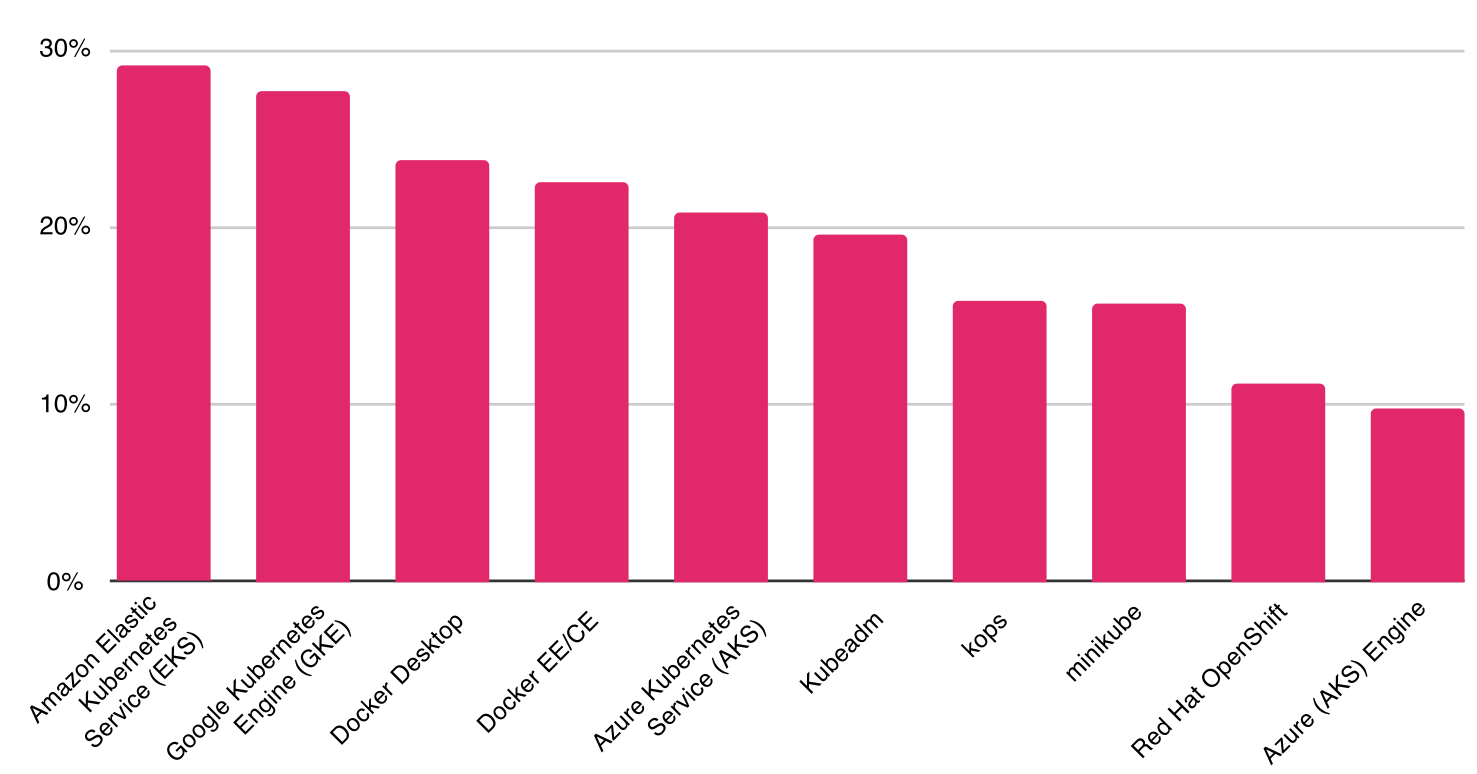
\includegraphics[width=16cm]{figures/cncf-2019-cont-tools.png}
    \captionsetup{justification=centering,margin=2cm}
    \caption{Top 10 tools used by organizations and companies to manage containers\cite{cncf-2019}}
\end{figure}

Further in this chapter, the methods categories (mentioned before) are briefly explained and a few methods are described in more detail. The focus is on \textbf{the two particular methods, which are used in the practical part of this work}:
\begin{itemize}
\item deploying on AWS, using AWS Managed Service (AWS EKS), using eksctl which is a AWS supported official tool,
\item deploying on AWS, not using any Managed Service, using Kops which is a command-line tool, not officially supported by any cloud, but designed exactly to deploy a Kubernetes cluster.
\end{itemize}

\subsection{Managed Services}
\textit{This section explains the term: Managed Services and lists some examples.}
\\

The complexity of Kubernetes infrastructure has a steep learning curve. Thus, a new market of services emerged: Managed Services. Managed Services are offered \textbf{to free the Kubernetes users of the burden of having to configure and maintain the not trivial Kubernetes infrastructure}. They provide a version of Kubernetes which is hosted and managed by a cloud\cite{article-managed}.

Managed services \textbf{offer a ready to use cluster}. The \textbf{popular Managed Kubernetes Services}, offered by major cloud providers, are:
\begin{itemize}
\item Elastic Kubernetes Service (Amazon EKS)\cite{online-eks}
\item Google Kubernetes Engine (GKE)\cite{online-gke}
\item Azure Kubernetes Service (AKS)\cite{online-aks}
\end{itemize}

\begin{figure}[H]
    \centering
    
\includegraphics[width=10cm]{figures/managed-k8s.png}
    \captionsetup{justification=centering,margin=2cm}
    \caption{The logos of three Managed Kubernetes Services, offered by the major cloud providers}
\end{figure}

Managed Services are \textbf{deeply integrated with other resources offered by a particular cloud}. For example: AWS EKS is claimed to integrate with AWS services like: Amazon CloudWatch, Auto Scaling Groups, AWS Identity and Access Management (IAM), Amazon Virtual Private Cloud (VPC), and AWS App Mesh\cite{online-eks}. A nice feature of AKS is integrated continuous integration and continuous delivery (CI/CD) experience\cite{online-aks}. Moreover, GKE is advertised as offered with "integrated Cloud Monitoring with infrastructure, application, and Kubernetes-specific views"\cite{online-gke}.

\textbf{Managed Services are relatively new}. For example, the initial release of AWS EKS happened at 05.06.2018\cite{eks-history}. Thus, some literature may not acknowledge its existence, e.g. the book "Mastering Kubernetes"\cite{book-mastering-k8s}. Another effect of the Managed Services being so young is that, to the best of this work's author knowledge, there is no other formal study which compares the two chosen methods of Kubernetes cluster deployment, from a perspective of satisfying production environment requirements. There was, however, an interesting study conducted which compares three Managed Kubernetes Services (the three mentioned above: AWS EKS, AKS and GKE) from a performance perspective\cite{article-managed}.

\subsection{Command-line tools designed exactly to deploy a Kubernetes cluster}
\label{cli-tools-to-k8s}
\textit{In this section, several opensource command-line tools are discussed. These tools are not supported by any particular cloud provider, but they are designed exactly to fulfill one aim: to deploy a Kubernetes cluster.}
\\

Github.com is a popular (used by many people) website which hosts code repositories. Many of those repositories are opensource.  Github.com uses a star-rating system: whenever someone likes a particular project, one can give it a star. Thus, \textbf{the number of stars given to a project may be used as a popularity measure} of a particular project.

Searching through Github.com, there are several \textbf{command-line tools available which exist only to fulfill one aim: to deploy a Kubernetes cluster}. The names of a few of the most popular of these projects, together with the amount of stars they were acclaimed with, are presented on the image below.

\begin{figure}[H]
    \centering
    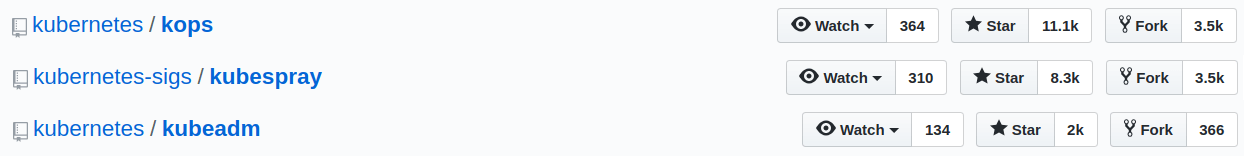
\includegraphics[width=17cm]{figures/custom-tools.png}
    \captionsetup{justification=centering,margin=2cm}
    \caption{Selected opensource tools which deploy a Kubernetes cluster, found on Github.com, state for date: 20.04.2020}
\end{figure}

The most popular tool amongst the four above is: \textbf{Kops}. Kops stands for Kubernetes Operations and on its Github.com page it is advertised as "the easiest way to get a production grade Kubernetes cluster up and running"\cite{online-kops-gh}. It is a command-line tool which allows to create, destroy, upgrade and maintain production-grade, highly available, Kubernetes clusters. It supports multiple clouds: AWS (officially), GCE and OpenStack (in beta support) and VMware vSphere (in alpha)\cite{online-kops-gh}. Furthermore, it can be used from multiple operating systems: Linux, Mac and Windows\cite{online-kops-install}. Kops is one of the recommended ways to setup a Kubernetes cluster and it is a tool which can be used to a create a producttion environment\cite{book-devops-with-k8s}

The second most popular tool is \textbf{Kubespray}. It also supports multiple clouds: AWS, GCE, Azure, OpenStack, vSphere, Oracle Cloud Infrastructure (Experimental), and Baremetal\cite{online-ks}. Furthermore, it also supports Highly Available deployment. The main difference between Kubespray and Kops is that \textbf{Kubespray uses Ansible} (an opensource tool to provision infrastructure) while \textbf{Kops performs the provisioning and orchestration itself}. Kops also provides more features tightly integrated with specified clouds\cite{online-ks-comp}.

There is also \textbf{kubeadm}. In contrast to Kops and Kubespray, kubeadm helps to get a minimum viable cluster "in a user friendly way". Furthermore, its scope is limited to the local filesystem\cite{online-kubeadm}. Kubernetes (and kubeadm) maintainers state that kubeadm is supposed to become a building block for all Kubernetes deployments. They also want to identify the common phases of a cluster deployment and make kubeadm an easy-to-use and configurable set of commands for each of those phases. An example of a common phase could be: certificate distribution\cite{kubeadm-vision-2017}.

Other than these three briefly described tools, \textbf{there are many more}, for instance: kube-aws\cite{kube-aws} or minikube\cite{minikube}. But neither listing them all nor describing them is needed for the purpose of this work. In the empirical part of this work, only one of the described tools is used: Kops.

\subsection{Custom solutions}
\textit{In this section, custom solutions for a Kubernetes cluster deployment are presented.}
\\

There is always a way to do (almost) everything on one's own. Here, one can split the deployment into two phases: infrastructure creation and, then, provisioning. To create infrastructure, meaning: virtual machines (compute resources), network and storage resources, one can use the following tool: \textbf{Terraform}. It is a tool made by Hashicorp, which incorporates \textbf{Infrastructure as Code}, in order to manage infrastructure. It has a CLI and thus it is fairly easy to use with a Continuous Integration server. Thanks to declarative configuration files, the resultant infrastructure is easy to reproduce\cite{terraform}. IaC facilitates future repetition of any work done with Terraform and thus any evaluations of this tool (done by experimenting with it) may be repeated in the future.

Terraform supports many providers, meaning that it can manage infrastructure of different public and private clouds (like: AWS, GCP, Azure, OpenStack) and, it can also handle local operations\cite{terraform}. There are also some alternative solutions, e.g.: \textbf{Heat or CloudFormation}. They support declarative configuration files too. But they are not cloud-agnostic. Heat is a solution for OpenStack cloud and CloudFormation - for AWS. Sometimes, there is a need to use many various providers in order to build an infrastructure and then, one may view it as a nice feature, to be able to use a unified syntax, which Terraform provides\cite{terraform-vs}.

After the infrastructure is created, the next step is to provision it. This step involves installing needed software (in this case: Kubernetes) and configuring it. However, since Kubernetes cluster is not just one machine, it would be tremendously tedious to provision each machine one by one manually. Thus, a chosen Configuration Management tool should be applied. There are any opensource tools available, some have been already presented in the section: \ref{Automation as production environment requirements}.

There was a time, when \textbf{Kubernetes source code contained SaltStack code}, in order to provision a cluster. The code can be still found on github: \url{https://github.com/kubernetes/kubernetes/tree/release-0.13/cluster/saltbase/salt}. However, now this method is deprecated (as can be read e.g. on this page: \url{https://github.com/kubernetes/kubernetes/tree/v1.18.2/cluster/}).

The advantage of such a custom solution is that it is very customizable and that, by making it work, one can learn Kubernetes in depth. On the other hand, it is not nearly as fast to design and first run as Managed Services. If one would like to immerse into the ocean of Kubernetes knowledge base, another great idea could be to try Kubernetes The Hard Way\cite{k8s-thw}.


\subsection{Deployment method: on AWS EKS Managed Service using eksctl}
\textit{Here is briefly described the first of the two methods, which are used in the empirical part of this work.}
\\

The goal of this method is to have the Kubernetes control plane managed by AWS. This means that it is AWS which is responsible for managing Kubernetes master components, such as: API Server, kube-scheduler, kube-controller-manager and also Etcd. The \textbf{control plane should be already highly available}, thanks to being deployed across \textbf{multiple Availability Zones}\cite{what-is-eks}. Availability Zone (AZ) is an isolated geographically place to host Amazon data centers. Several AZs create a Region. AZs in a Region are connected through low-latency links\cite{az}.

The control plane being already highly available means that there should be at least two API server nodes and three etcd nodes that run across three Availability Zones within a Region. In addition, AWS EKS is responsible for automatically detecting and replacing unhealthy control plane instances. Furthermore, version upgrades should be provided automatically and applied\cite{what-is-eks}. There exists a \textbf{Service Level Agreement (SLA)} especially concerning AWS EKS. It is a policy which governs the use of the Amazon Elastic Container Service for Kubernetes. For example, the SLA states what is the Monthly Uptime Percentage during any monthly billing cycle (at least 99.95\%)\cite{eks-sla}. Thanks to such a SLA, AWS EKS is claimed to be \textbf{reliable and recommended for production workloads}\cite{what-is-eks}.

As far as the master components are concerned, they are run in an account managed by AWS. The Kubernetes API is exposed via the Amazon EKS endpoint which is associated with the cluster. Each Amazon EKS cluster control plane runs on its own set of Amazon EC2 instances\cite{eks-clusters}.

Furthermore, AWS EKS also manages the Kubernetes (worker) nodes. The nodes are run in one's AWS account and AWS connects them to the already deployed control plane via the cluster API server endpoint. The worker nodes are grouped in an AWS EC2 Auto Scaling group. The latter fact has some consequences, namely all these nodes have to\cite{eks-worker}:
\begin{itemize}
\item use the same Amazon EC2 instance type,
\item be instantiated from the same Amazon EC2 image (called: AMI, an abbreviation from Amazon Machine Image\cite{aws-ami}),
\item use the same Amazon EKS worker node IAM role.
\end{itemize}

Fortunately, an AWS EKS cluster can contain multiple node groups, therefore there is a possibility to utilize nodes of various AMIs\cite{eks-worker}. This is an important information, because a Kubernetes administrator may be interested in choosing a particular operating system for a node. There exist such AMIs, which are specifically designed for EKS. This AMI is built on top of Amazon Linux 2 and has some essential tools installed and configured: Docker, kubelet, and the AWS IAM Authenticator. The way in which the AMI is built is coded and made opensource. Thanks to this solution, everyone can build their own AMI, basing on the opensource version\cite{eks-optimized-ami}. There is even an option to have Windows worker nodes\cite{eks-worker-win}.

The cluster control plane is fronted by \textbf{an Elastic Load Balancing Network Load Balancer} and also all the networking is taken care of (elastic network interfaces are provisioned in VPC subnets) to provide connectivity from the control plane instances to the worker nodes. Thanks to that, the AWS EKS \textbf{user can access the Kubernetes API Server}\cite{eks-clusters}.

In order to use AWS EKS, there are two ways supported:
\begin{itemize}
\item using eksctl CLI,
\item using AWS Management Console and AWS CLI.
\end{itemize}

Both of them demand installing AWS CLI. In this work, \textbf{the method with eksctl CLI is applied}. Eksctl is officially the CLI for AWS EKS, endorsed by AWS, though it was launched by WeaveWorks. With eksctl, one can use a simple command to instantiate the whole cluster\cite{eks-cli-official}:
\begin{lstlisting}[basicstyle=\small,caption={A command of eksctl CLI tool used to create a Kubernetes cluster},captionpos=b,language=Bash,xleftmargin=1cm]
$ eksctl create cluster
\end{lstlisting}

The cluster can be \textbf{configured with a YAML file and also by setting eksctl CLI flags}. The documentation describing how to do it, is presented on the official eksctl website\cite{eksctl}. There is also an example YAML configuration file attached on that website. This file is used to customize a cluster. It is also appended below.

\begin{lstlisting}[basicstyle=\tiny,caption={An example YAML file used to customize a Kubernetes cluster created with eksctl CLI tool\cite{eksctl}},captionpos=b,language=Bash,xleftmargin=1cm]
apiVersion: eksctl.io/v1alpha5
kind: ClusterConfig

metadata:
  name: basic-cluster
  region: eu-north-1

nodeGroups:
  - name: ng-1
    instanceType: m5.large
    desiredCapacity: 10
  - name: ng-2
    instanceType: m5.xlarge
    desiredCapacity: 2
\end{lstlisting}

This example configuration file sets a name for the cluster ('basic-cluster'), chooses an Amazon Region in which all the AWS resources will be deployed ('eu-north-1') and also configures the details of Kubernetes nodes. Many more options can be set.

After the cluster is created and after a connectivity with a Kubernetes cluster endpoint is established, it is now possible to deploy applications on top of the cluster. The illustration below depicts the stages of working with AWS EKS.
\begin{figure}[H]
    \centering
    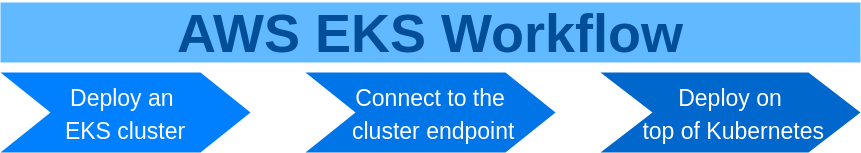
\includegraphics[width=12cm]{figures/eks-workflow.png}
    \captionsetup{justification=centering,margin=2cm}
    \caption{A schema presenting the stages of working with AWS EKS}
\end{figure}

Much more information on how to deploy AWS EKS Kubernetes cluster can be found. The official websites of AWS EKS\cite{what-is-eks} and eksctl\cite{eksctl} are a great source of help. More examples of cluster configuration can be found on the official eksctl page on Github.com\cite{eks-gh}. A sample Kubernetes use cases scenarios, for example: creating a CI pipeline to deploy a sample Kubernetes service, can be found in the Internet\cite{eksworkshop}.


\subsection{Deployment method: on AWS using Kops}
\textit{Here is briefly described the second of the two methods, which are used in the empirical part of this work.}
\\

Kops was already introduced in the section: \ref{cli-tools-to-k8s}. Similarly to eksctl, Kops can also create a Highly Available Kubernetes cluster. However it demands more work than eksctl. The commands which allow to create a cluster on AWS is\cite{book-mastering-k8s}:
\begin{lstlisting}[basicstyle=\small,caption={The commands of Kops CLI tool used to create a Kubernetes cluster configuration and then to deploy the cluster},captionpos=b,language=Bash,xleftmargin=1cm]
$ kops create cluster ${CLUSTER_NAME} --state "s3://${K8S_EXP_KOPS_S3_BUCKET}" --cloud=aws --zones=us-east-1c
$ kops update cluster ${CLUSTER_NAME} --state "s3://${K8S_EXP_KOPS_S3_BUCKET}" --yes
\end{lstlisting}
But, before these commands can be run, one has to provide some minimal DNS configuration via Route53 (an AWS resource responsible for networking), set up a S3 bucket (another AWS resource, responsible for storage) to store the cluster configuration\cite{book-mastering-k8s} and also configure the AWS IAM user (an AWS resource responsible for access management) and create a SSH key pair\cite{online-kops-aws}. The instructions explaining how to set up the AWS resources are provided on the official Kops website\cite{online-kops-aws}.

The configuration of Kops is kept in an S3 bucket. In order to change the configuration, one has to enter the following command\cite{online-kops-aws}:
\begin{lstlisting}[basicstyle=\small,caption={A command of Kops CLI tool used to edit a Kubernetes cluster configuration},captionpos=b,language=Bash,xleftmargin=1cm]
$ kops edit cluster ${NAME}
\end{lstlisting}

A configuration spec file is generated during the create phase and uploaded to a S3 bucket. The configuration can be also kept in YAML file. All the configuration options are available on a Kops Golang documentation website\cite{online-kops-yaml-config-golang}. A cluster can be created then in the following way\cite{online-kops-yaml-config}:
\begin{lstlisting}[basicstyle=\small,caption={A command of Kops CLI tool used to create a Kubernetes cluster using a YAML configuration file},captionpos=b,language=Bash,xleftmargin=1cm]
$ kops create -f $NAME.yaml
\end{lstlisting}


The stages of working with a Kubernetes cluster deployed on AWS with Kops are similar to the stages of working with eksctl, but there is the additional first stage. It is depicted on the below schema.
\begin{figure}[H]
    \centering
    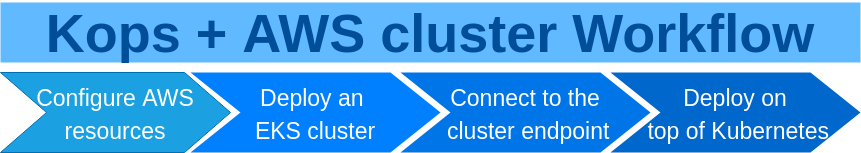
\includegraphics[width=12cm]{figures/kops-aws-workflow.png}
    \captionsetup{justification=centering,margin=2cm}
    \caption{A schema presenting the stages of working with a Kubernetes cluster deployed on AWS with Kops}
\end{figure}

The next stage, after instantiating a cluster is to connect to it through an endpoint. Such configuration is automatically generated and written to '~/.kube/config' (on Linux Operating System)\cite{online-kops-aws}. The same is true also for AWS EKS.

Kops has been around a long time as an AWS-specific tool, but now it also supports other clouds\cite{book-cndwk}\cite{online-kops-gh}. Its main features such as: automated Kubernetes cluster deployment, highly available master or adding a variety of custom Kubernetes addons\cite{kops-addons} indicate that Kops is an attractive tool, worthy to at least try out.

There are many Internet sources available to broaden one's knowledge about Kops: the official Kops website\cite{online-kops}, the Kops project website on Github.com\cite{online-kops-gh} and there are also some comparisons of Kops versus alternative tools available, e.g.: "A Multitude of Kubernetes Deployment Tools: Kubespray, kops, and kubeadm"\cite{online-kops-blog}.

\subsection{Amazon services allowing to run containers}
\textit{In order to exhaust the topic of the Amazon services which allow to run containers, this chapter was created. This chapter shortly characterizes each such AWS Service.}
\\

Below, all the AWS Services, used to manage containers, are listed:
\begin{itemize}
\item AWS ECS
\item AWS ECR
\item AWS Fargate
\item AWS EKS
\end{itemize}

\textbf{AWS ECS} stands for Amazon Elastic Container Service. It is a service that provides \textbf{a highly secure, reliable, and scalable way to run containers}. Secure, because the containers are run in a custom VPC (Virtual Private Cloud). Thanks to that, custom firewall rules can be applied to the containers (by using AWS Security Groups). Furthermore, each of the containers uses IAM, which means that access to each container can be restricted and granular access permissions can be assigned. Running containers on ECS is reliable thanks to the SLA, which guarantees a Monthly Uptime Percentage of at least 99.99\%\cite{ecs}.

\textbf{AWS ECR} is an abbreviation from Amazon Elastic Container Registry. It is not a service which strictly manages the containers, but it manages images. It is \textbf{a fully-managed Docker container registry}. AWS ECR eliminates the need to run such a registry on-premises or worry about scaling the underlying infrastructure. The images are hosted in a highly available and scalable architecture. Similarly to AWS ECS, AWS ECR also integrates with IAM\cite{ecr}.

\textbf{AWS Fargate is a serverless service to run containers}. This service is responsible for allocating the right amount of compute, eliminating the need to choose instances and scale cluster capacity. It can work with both: AWS ECS and AWS EKS. AWS Fargate runs each task or pod in its own kernel, therefore the tasks and pods are provided with their own isolated compute environment. Without Fargate, the containers are run on EC2 instances, so the end user has to pay for both: an EC2 instance and for an ECS container\cite{fargate}. Running serverless Kubernetes Pods Using Amazon EKS and AWS Fargate is very new, a blog post informing about this possibility was created at 3rd of December 2019\cite{fargate-for-eks}.

The last service on the list above, \textbf{AWS EKS}, was already described in this chapter.

\subsection{Summary}

There are \textbf{many methods of deploying a Kubernetes cluster}. According to the authors of "Cloud Native DevOps with Kubernetes"\cite{book-cndwk}, the best solution is to use \textbf{Managed Services}. The authors argue that, thanks to this method, one can get a fully working, secure, highly available, production-grade cluster in a few minutes and for a little price. Managed Services are certainly a good way to try Kubernetes out. Then, if one wants to do something non-standard or to experiment with the cluster, then one could choose \textbf{a custom or a hybrid solution}. The self-hosted, deployed on-premises way is recommended if the following qualities are of a great importance: price, low-network latency, regulatory requirements and total control over hardware\cite{book-mastering-k8s}.

Managed Services offer many features like: built-in autoscaling, security, high availability, having serverless options. However, they may be more expensive (for example, when using AWS EKS, one has to pay \$0.10 per hour for each Amazon EKS cluster\cite{online-eks-pricing}) and less customizable. Custom solutions allow the Kubernetes administrator to broaden their knowledge and \textbf{grasp the deep understanding} on what is going on under the Kubernetes hood (i.e. one can customize how the Kubernetes control plane is deployed or set up a custom network topology).

There is \textbf{no one right answer} which fits all the use cases. It is always advised to do one's own research and to try and experiment with the existing methods.

\newpage

% 4
\setcounter{figure}{0}
\setcounter{table}{0}
\setcounter{lstlisting}{0}
% 4
\section{Preparations for production deployment of a Kubernetes cluster}
\label{prep-prod}
\textit{This is a practical section. It includes planning and designing the production deployment, considering: capacity planning, choosing which requirements to satisfy and taking any other deployment and infrastructure related decisions. No AWS resources were created here, but AWS CLI was used to get some information.}
~\\

\subsection{AWS Region}
\textit{The first decision to take is to choose the AWS Region in which all the resources should be deployed.}
\\

The Kubernetes cluster deployment constitutes the empirical work of this study. The deployment will target the AWS cloud. This cloud provides many data centers, spread across multiple physical locations around the world. AWS calls these locations: Regions, Availability Zones, and Local Zones. AWS offers many resources (for example: S3, EC2 or EKS). Some of them are global, whereas the others are tied to a Region, an Availability Zone, or a Local Zone\cite{az}.

While it matters not which Availability Zone will be chosen, \textbf{choosing a Region has some consequences}. For example, AMIs are tied to a Region. AMIs may be copied between Regions. It may happen, that some officially supported AMIs are available only in a limited number of Regions and choosing some other Region would incur more \textbf{time and money} needed to copy the image. There is a charge for data transfer between Regions\cite{az}.

AWS Local Zones are a new type of AWS infrastructure deployment. Thanks to them, AWS resources can be put closer to large population, industry, and IT centers where no AWS Region exists today. AWS Local Zones help to run latency sensitive applications closer to end users. Even single-digit millisecond latency can be achieved. The use cases for such latency are for example: media & entertainment content creation, real-time gaming, reservoir simulations, electronic design automation, and machine learning\cite{lz}. AWS Local Zones are available since 9th March 2020 and there is currently one AWS Local Zone, available in Los Angeles, California\cite{lz-blog}. For this work, single-digit millisecond latency is not needed.

In this work, AWS EC2 instances will be used (Elastic Compute Cloud resources). The following AWS CLI command was run to list all the available regions for the AWS account of the author of this work:
\begin{lstlisting}[basicstyle=\small,caption={A command of AWS CLI tool used to list all the available regions (for an AWS account)},captionpos=b,language=Bash,xleftmargin=1cm]
$ aws ec2 describe-regions
\end{lstlisting}

The returned list of Regions was: "eu-north-1", "eu-west-3", "eu-west-2", "eu-west-1", "eu-central-1", "ap-south-1", "ap-northeast-2", "ap-northeast-1", "sa-east-1", "ca-central-1", "ap-southeast-1", "ap-southeast-2", "us-east-1", "us-east-2", "us-west-1", "us-west-2". Considering the geographical proximity, the Region should be in Europe. The Regions' names are mapped to geographical locations below (limited to Europe)\cite{aws-region-map}:
\begin{itemize}
\item "eu-north-1" - Europe (Stockholm)
\item "eu-west-1" - Europe (Ireland)
\item "eu-west-2" - Europe (London)
\item "eu-west-3" - Europe (Paris)
\item "eu-central-1" - Europe (Frankfurt)
\item "eu-south-1" - Europe (Milan)
\end{itemize}

The next criterion of choosing the Region is \textbf{price}. The pricing for EC2 instances were compared for 5 AWS Regions (available for a particular AWS account, in Europe). A few EC2 instance types were considered, but from the General Purpose family of types. Only Linux/UNIX usage was taken into consideration. The comparison is presented in the table below. The data comes from the official AWS EC2 pricing website\cite{ec2-pricing}. The prices are noted \textbf{in USD per hour of an EC2 instance running}.

\begin{table}[H]
\begin{tabularx}{0.9\textwidth} {
  | >{\centering\arraybackslash}X
  | >{\centering\arraybackslash}X
  | >{\centering\arraybackslash}X
  | >{\centering\arraybackslash}X
  | >{\centering\arraybackslash}X
  | >{\centering\arraybackslash}X | }
 \hline
  \textbf{Instance Type} & \textbf{London} & \textbf{Ireland} & \textbf{Frankfurt} & \textbf{Paris} & \textbf{Stockholm}  \\
 \hline
 t2.nano  & 0.0066 & 0.0063 & 0.0067 & 0.0066 & not given \\
 \hline
 t2.micro  & 0.0132  & 0.0126 & 0.0134 & 0.0132 & not given \\
 \hline
 t2.small  & 0.026 & 0.025 & 0.0268 & 0.0264 & not given \\
 \hline
 t2.medium  & 0.052 & 0.05 & 0.0536 & 0.0528 & not given \\
 \hline
\end{tabularx}
\caption{\label{tab:ec2-pricing}Comparison of the price, noted in USD, of 1 hour running of an EC2 instance on AWS, considering a few selected AWS Regions. Based on the official AWS EC2 pricing website\cite{ec2-pricing}}
\end{table}


Thus, basing on the three factors (Region being available for an AWS account, in Europe and the cheapest) - \textbf{the Region chosen is: Europe (Ireland) - "eu-west-1"}. Then, the next thing to decide upon was choosing availability zones. All the AZs available in the chosen region can be listed with the following command\cite{online-kops-aws}:
\begin{lstlisting}[basicstyle=\small,caption={A command of AWS CLI tool used to list all the available AZs in the chosen AWS Region)},captionpos=b,language=Bash,xleftmargin=1cm]
$ aws ec2 describe-availability-zones --region eu-west-1
\end{lstlisting}
The command output listed the following AZs: "eu-west-1a", "eu-west-1b", "eu-west-1c".

\subsection{Version of Kubernetes}
\textit{In this section, it is decided which Kubernetes version to use.}
\\

\subsubsection{Why it is important to choose a particular version}
In order to compare two methods of Kubernetes deployment in a reasonable way, \textbf{both methods should deploy the same Kubernetes version}. Also, the version should be one of the latest released ones, for the sake of keeping this comparison up-to-date. Furthermore, using a specified version is important for the production environment, because:
\begin{itemize}
\item the environment should be easy to recreate,
\item the experiment (the empirical work of this study: deploying a Kubernetes cluster) should be possible to be repeated,
\item using specified versions helps to incorporate Infrastructure as Code and DevOps best practices and to automate the deployments.
\end{itemize}

\subsubsection{Which version was chosen}
At the time of writing this work, \textbf{in May 2020}, the latest released versions of the needed software are:
\begin{itemize}
\item Kubernetes version 1.18\cite{online-k8s-blog-latest},
\item Kops version 1.16.2, Kubernetes versions supported by Kops are: 1.16, 1.15, 1.14, 1.13, 1.12\cite{online-kops-versions}\cite{kops-releases},
\item Kubernetes versions supported by EKS: 1.16.8, 1.15.11, 1.14.9, 1.13.12. However, Kubernetes version 1.13 is deprecated\cite{online-eks-versions}. There are also particular EKS Platform versions for each supported Kubernetes version. For example, for Kubernetes 1.16.8 there is one EKS Platform version: eks.1\cite{online-eks-platform-versions}.
\item Eksctl version is 0.20.0\cite{online-eksctl-versions}
\end{itemize}

EKS documentation recommends that unless a specific Kubernetes version is required, the latest supported version should be chosen\cite{online-eks-versions}. Basing on the above information, \textbf{the maximum version of Kubernetes, supported by the two deployment methods, was: v1.16.8}. However, one has to consider the AWS AMIs with Kubernetes installed. There are some EKS-optimized Linux AMIs - built for this exact purpose - to be deployed in a Kubernetes cluster. They are built on top of \textbf{Amazon Linux 2}\cite{eks-optimized-ami}. Besides the official Amazon EKS-optimized AMIs, Canonical (the commercial support provider for Ubuntu) has partnered with Amazon EKS to create worker node AMIs built on top of \textbf{Ubuntu}\cite{eks-ubu}. Judging from the official Canonical website, which provides the EKS Ubuntu AMIs IDs, the latest supported Kubernetes version is 1.15. There is an AMI available for the chosen AWS Region "eu-west-1" and the AMI's ID is: ami-0ceab0713d94f9276\cite{eks-ubu-ami-id}.

Amazon Linux 2 is a Linux Server Operating System, provided by Amazon. Among the features it provides are: optimized performance (to help ease integration with AWS Services), long term support, bleeding edge software updates support, on-premises use, systemd support, etc.\cite{al2}. However, Amazon Linux 2 is a RPM-based Linux distribution (which can be judged based on information that many applications developed on CentOS (and similar distributions) run on Amazon Linux)\cite{al2-centos}. RPM-based Linux distributions include: CentOS, Fedora, Red Hat Linux, etc. Since the author of this work has little experience with RPM-based Linux distributions, \textbf{the AWS EKS AMIs with Ubuntu were preferred}. This decision should not impact the aim of this work but it should result in less time spent on troubleshooting.

Considering all the information presented in this section, the \textbf{version of Kubernetes chosen was: 1.15.11}.


\subsection{Capacity planning}
\textit{Here the needed capacity is discussed. The aim is to have a minimal working cluster that could be representative for a production environment.}
\\

The important thing is, that the to-be-deployed Kubernetes cluster, should have the minimal amount of capacity, but still it should be representative for a production environment. Here \textbf{chicken-counting} (0, 1, many) comes to the rescue. Applying the chicken-counting technique means that if a production site has 250 web servers, 2 should be enough to represent it\cite{book-cicd}. Since a Kubernetes cluster consists of a master node and worker nodes, then it was decided that \textbf{a representative cluster would be made of one master node and two worker nodes}.

The capacity of a cluster means the sum of CPU and memory of all the cluster worker nodes. Multiple ways are possible to achieve the desired target capacity. Example given: if a cluster with a total capacity of 8 CPU cores and 32 GB of RAM is needed, then it can be achieved by, for example, having two nodes (each with 4 CPU and 16 GB RAM) or having four nodes (each with 2 CPU and 8 GB RAM)\cite{kubernetes-node-size}. Now there are two questions:
\begin{itemize}
\item it is better to have a few bigger nodes or many smaller nodes?
\item what is the minimal capacity needed for a production cluster?
\end{itemize}

The table below summarizes the advantages and disadvantages of having a few bigger nodes. For more information about the pros and cons presented in the table \ref{tab:pros-cons-large-nodes}, a reader is referred to an online source: "Architecting Kubernetes clusters — choosing a worker node size"\cite{kubernetes-node-size}.

\begin{table}[H]
\begin{tabularx}{1\textwidth} {
  | >{\centering\arraybackslash}X
  | >{\centering\arraybackslash}X | }
 \hline
  \textbf{Advantages} & \textbf{Disadvantages}  \\
 \hline
 Less management overhead (less number of machines to manage)  & Large number of pods per node (each pod introduces some overhead, if there are too many pods, the system may slow down)   \\
 \hline
 Resource-hungry applications allowed  & Large scaling increments  \\
 \hline
  Potential lower costs per node (the price increase for a more powerful may not be linear)  & Limited replication (each replica of a pod may be requested to be deployed on a different node. If a HA application requires 5 replicas, but there are only 2 nodes in a cluster, then the effective degree of replication is reduced to 2)  \\
 \hline
  Large numbers of nodes can be a challenge for the Kubernetes control plane (there are many network communication paths and also also more load on the etcd database) & The impact of one failed node is big   \\
 \hline
  Better resources utilization &   \\
 \hline
\end{tabularx}
\caption{\label{tab:pros-cons-large-nodes}Comparison advantages and disadvantages of having a few bigger nodes in a Kubernetes cluster instead of having many smaller nodes\cite{kubernetes-node-size}}
\end{table}

However, in the Internet there are contradictory information about the limited replication. The online source cited above\cite{kubernetes-node-size} states that there can be maximally as many replicas as worker nodes in a cluster, while another source - a blog post\cite{learnk8s-ll} claims that there can be more pod replicas than nodes. This information was not verified in practice in this work. Perhaps the replicas limit depends on Kubernetes version - but this is just a speculation of this work's author.

It is officially claimed, that Kubernetes supports up to 5000 nodes and up to 100 pods per node\cite{kubernetes-node-size}\cite{kubernetes-large}. However, in practice, 500 nodes may already lead to non-trivial challenges. Furthermore, as far as AWS EKS is concerned, there are some hard limits for number of pods allowed for a particular EC2 instance type. For example, for a t2.medium instance, the maximum number of pods is 17, for t2.small it's 11, and for both: t2.micro and t2.nano it's 4\cite{kubernetes-node-size}\cite{eks-hard-limits}.

\textbf{There was no official statement found stating the minimal capacity of a Kubernetes cluster}. Thus, the EC2 instance type for a Kubernetes worker nodes should depend on the resources needed by the pods. (Some pods will be deployed in order to test whether the cluster is healthy). Some overhead must be also considered, because the amount of compute resources that are available for pods, \textbf{the allocatable}, is smaller than the capacity of the whole node\cite{k8s-alloc}.

\subsection{Tools and development environment}
\label{tools}
\textit{This section can be treated as a checklist of what tools should be gathered before deploying a Kubernetes cluster. It also characterizes a development environment.}
\\

Let's start with a list of essential tools needed:
\begin{itemize}
\item Linux
\item bash
\item kubectl
\item aws cli 2
\item eksctl
\item kops
\item helm
\item bats-core
\end{itemize}

Now, each of these tools will be briefly introduced. TODO

When it comes to \textbf{development environment} - the Ubuntu 18.04 workstation was used. In order to facilitate repetition of the empirical work of this study, all the deployment was performed from a Docker container. Thus, the local development environment was just obliged to: have Docker installed, Internet access and AWS credentials configured. The Docker container used, was created from a Docker image: TODO, ... Dojo, Dojofile contents, , dojo out of scope of this work, how the container was run, etc... Thanks to such a solution, it should be easy to run the deployment from a local workstation (e.g. from a local laptop) and also from a CI server.

TODOooo


\subsection{Selected requirements of a production deployment and acceptance criteria needed to satisfy them}
\textit{Here a set of production deployment requirements is presented. Each of them is shortly described. Acceptance criteria, needed to satisfy the requirements are provided. This section helps to plan the deployment.}
\\

\textbf{There are numerous requirements for a production deployment of a Kubernetes cluster}. Some of them were gathered throughout the available literature and presented in the section: \ref{Production deployment requirements}. It is common knowledge that companies, which deploy Kubernetes and similar systems, obey some set of best practices, dedicated to these companies only. Thus, the requirements presented in this work do not exhaust the topic.

Below, there is a list of the selected production deployment requirements. In the empirical part of this study, the requirements were  attempted to be satisfied.
\begin{itemize}
\item A healthy cluster
\item Automated operations
\item Central Logging
\item Central Monitoring
\item Central Audit
\item Backup
\item High Availability
\item Autoscaling
\item Security
\item Live Cluster Upgrades
\end{itemize}

The set entails \textbf{10 requirements}. Each of them was already described theoretically, but further in this chapter, each requirement is explained from a practical point of view. The \textbf{acceptance criteria} needed to satisfy each of the requirements are presented. Basing on this, a plan of a Kubernetes cluster deployment is created. The work done is described in the next chapter, together with any problems encountered and troubleshooting sessions.

\subsubsection{A healthy and usable cluster}
\label{A healthy cluster}

% health checks
Unless any of the Kubernetes control plane components is healthy, it will need to be fixed. It should not be a problem with a managed Kubernetes services, but for self hosted clusters, this should be checked. It should be noted that, since the \textbf{health checks} ought to be run frequently, they shouldn't do anything too expensive. To monitor the health of a Kubernetes cluster, \textbf{the following could be checked: number of nodes, node health status, number of pods per node and overall, resource usage/allocation per node, and overall}\cite{book-cndwk}.

% api endpoint reachable under a domain name
When all the cluster health checks are passed, then the cluster is healthy. But, the cluster should be also usable for end users. End users will want to deploy applications on top of the cluster. Thus, they have to have the possibility to reach the cluster endpoint, which in practice means, that they have to \textbf{be able to reach the Kubernetes API Server endpoint}. Such an endpoint may be an IP address or a domain name. Since the cluster will be deployed in a production environment, a domain name is preferred. Furthermore, many sources claim that a top-level domain or a subdomain is required to create a Kubernetes cluster with Kops. Alternatively, gossip-based DNS can be used instead, and then, the cluster domain name would have to end with \textit{.k8s.local} and the API server would be available under the AWS load balancer address\cite{kops-howto-aws}\cite{online-kops-aws}\cite{kops-howto-k8s}\cite{kops-gossip}.

% test app can be deployed
TODO: deploy some test app and test it

To summarize, in order for a cluster to be healthy and usable, the following acceptance criteria must be met:
\begin{itemize}
\item the cluster should have health checks passed,
\item the Kubernetes API Server endpoint should be reachable for the end users under a domain name,
\item it should be tested that an application can be deployed on top of a Kubernetes cluster.
\end{itemize}

* kubectl get nodes, kubectl version --short,
* deploy some test service and test it; use helm - maybe apache chart + use the idea from https://learnk8s.io/blog/kubernetes-chaos-engineering-lessons-learned to display the hostname of the current pod in a web page (so that we know if many pods are deployed?); kubectl scale then!
* use bats for all the tests
* kops validate cluster


% "Service: A Kubernetes Service that identifies a set of Pods using label selectors. Unless mentioned otherwise, Services are assumed to have virtual IPs only routable within the cluster network." thus we use ingress https://kubernetes.io/docs/concepts/services-networking/ingress/ ; "Kubernetes Service with type: LoadBalancer -> Each Service spawns its own ELB, incurring extra cost." https://medium.com/@dmaas/amazon-eks-ingress-guide-8ec2ec940a70


\subsubsection{Automated operations}

Setting up a package manager for reusable Kubernetes deployments is recommended\cite{gruntwork-howto-blog}. In this work: Helm is used and it was already described in the section: \rel{tools}.

* Automation and Infrastructure as Code - eksctl YAML config, kops YAML config, cloudformation? terraform?
* tasks file - one command to run one operation
* helm and bats also help automation
* additionally (if there is time): try AWS CI Server (or some other CI Server)
* write again that iac facilitates the repetition of future evalutaions, repeating this experiment

\subsubsection{Central Logging}

* try AWS CloudWatch Logs
* additionally (if there is time): deploy Graylog (or Fluentd or Logstash, etc) on AWS

\subsubsection{Central Monitoring}

* try AWS CloudWatch Alarms and dashboards
* try kubernetes dashboard
* additionally (if there is time): deploy Grafana + influxdb on AWS

\subsubsection{Central Audit}

* try AWS CloudTrail

\subsubsection{Backup}

* backup etcd with the test service deployed and try to restore in a new k8s cluster

\subsubsection{High Availability}

* it is probably already implemented, so just write about it
* additionally do: "How to move from single master to multi-master in an AWS kops kubernetes cluster" https://blenderfox.com/2018/01/23/how-to-move-from-single-master-to-multi-master-in-an-aws-kops-kubernetes-cluster/
* NAT Gateway

\subsubsection{Autoscaling}

* increase the number of pod replicas, make autoscaling work

\subsubsection{Security}
\textit{Security is handled by applying private networking, AWS Security groups, proper authentication and authorization.}
\\

First, let's handle the networking. In order to have a clear understanding of how the networking will be set up, a few terms have to be explained. \textbf{VPC stands for Virtual Private Cloud} and it is an AWS resource, providing the networking services. When a VPC is created, it means that a virtual private network is created and assigned to a particular AWS account. AWS resources can be launched into that VPC. Each VPC has a CIDR block assigned. The VPC cannot span more than one AWS Region. The VPC can be divided into subnetworks (or subnets). One subnet cannot span more than one Availability Zone. \textbf{Subnets can be either public or private}. If a subnet's traffic is routed to an internet gateway (which is an AWS resource), the subnet is known as a public subnet. Otherwise, a subnet is private\cite{aws-vpc}. This means that public subnets have access to the Internet.

In order to stay secure, access to the Kubernetes cluster should be limited. This can be achieved in multiple ways.

%%% aaa

it was decided that in the deployments for this work, \textbf{the private network topology was chosen}. This should be set for both deployment methods.


% private networking

There are \textbf{two network topologies supported by Kops: public and private}. When the public topology is chosen, then all masters and workers of a Kubernetes cluster will be launched in a public subnet in the VPC. Respectively: when using the private topology, all the machines will be launched in a private subnet in the VPC\cite{kops-net-topo}. This is settable as a CLI flag\cite{kops-net}:
\begin{lstlisting}[basicstyle=\small,caption={CLI flag used by kops to set private networking mode},captionpos=b,language=Bash,xleftmargin=1cm]
--topology private
\end{lstlisting}

When using eksctl, this is also possible: the initial nodegroup (worker nodes) can be isolated from the public Internet by the following CLI flag\cite{eksctl-net}:
\begin{lstlisting}[basicstyle=\small,caption={CLI flag used by eksctl to set private networking mode},captionpos=b,language=Bash,xleftmargin=1cm]
--node-private-networking
\end{lstlisting}
or by setting in the YAML configuration file\cite{eks-example}:
\begin{lstlisting}[basicstyle=\small,caption={YAML configuration used by Kops to set private networking mode},captionpos=b,language=Bash,xleftmargin=1cm]
nodeGroups:
  - name: ng-1
    instanceType: m5.xlarge
    desiredCapacity: 2
    privateNetworking: true # if only 'Private' subnets are given, this must be enabled
\end{lstlisting}

% HA NAT Gateway

When the private network topology is chosen, kops creates one NAT Gateway (NGW) per AZ\cite{kops-net2}. Such a \textbf{NGW is then highly available} - which is an important production deployment requirement. There is also a possibility to set it with eksctl with\cite{eksctl-net}:
\begin{lstlisting}[basicstyle=\small,caption={YAML configuration used by eksctl to set NAT Gateway as Highly Available},captionpos=b,language=Bash,xleftmargin=1cm]
vpc:
  nat:
    gateway: HighlyAvailable # other options: Disable, Single (default)
\end{lstlisting}

The NAT Gateway is needed, because the worker nodes must have access to the Internet, in order to function properly. If the worker nodes are deployed in a private subnet, then the private subnet will access the Internet through a NAT Gateway\cite{eks-net}.

% endpoint access

The next thing is to consider \textbf{whether the API Server is accessible from within a VPC only or from the public Internet}. For the production deployment, access from within a VPC only is recommended. \textbf{In order to allow access from a remote computer, through the Internet, a bastion host or a VPN server is needed}\cite{gruntwork-howto}. It is essential to understand that NAT Gateway is needed in order to allow Internet access from an AWS EC2 machine, while bastion host allows to access that machine from outside. The functionality of a bastion host is to provide secure access to Linux instances located in the private and public subnets\cite{aws-bastion}.

When a new EKS cluster is created, Amazon provides an endpoint for the managed Kubernetes API server. Thanks to that, one can communicate with the cluster (for example using a Kubernetes management tool: kubectl). As a default configuration, this API server endpoint is public to the internet, and also access to the API server is secured using a combination of AWS IAM (Identity and Access Management) and RBAC (native Kubernetes Role Based Access Control). Private access to the API server can be enabled. Thanks to that all communication between the worker nodes and the API server stays within a VPC\cite{eks-cluster-endpoint}.

When private endpoint is enabled, AWS EKS creates a Route 53 private hosted zone, but this zone does not appear in AWS Route 53 resources. What is essential is that the Route53 resource is assigned to a VPC and such a VPC must have 'enableDnsHostnames' and 'enableDnsSupport' set to 'true', and also the DHCP options set for the VPC must include 'AmazonProvidedDNS' in its domain name servers list. Apart from this, there is also a requirement that an IAM Role or User (used to manage the AWS EKS cluster) must be given 'route53:AssociateVPCWithHostedZone' permissions\cite{eks-cluster-endpoint}.

Enabling private endpoint is settable with eksctl in YAML file\cite{eksctl-net}:
\begin{lstlisting}[basicstyle=\small,caption={YAML configuration used by eksctl to set EKS cluster endpoints},captionpos=b,language=Bash,xleftmargin=1cm]
vpc:
  clusterEndpoints:
    publicAccess:  <true|false>
    privateAccess: <true|false>
\end{lstlisting}
However, if only private access is allowed, then eksctl cannot create the cluster. Thus, at cluster creation, both: public and private access will be enabled. Then, the public access can be disabled\cite{eksctl-net}.


services, ingress, public access, ALB - https://blog.gruntwork.io/how-to-build-an-end-to-end-production-grade-architecture-on-aws-part-1-eae8eeb41fec

https://kops.sigs.k8s.io/node_authorization/

a Defense in Depth strategy - https://blog.gruntwork.io/how-to-build-an-end-to-end-production-grade-architecture-on-aws-part-1-eae8eeb41fec

The table below summarizes what configuration must be set when using eksctl and kops to ensure a secure, production ready networking:

\begin{table}[H]
\begin{tabularx}{0.9\textwidth} {
  | >{\centering\arraybackslash}X
  | >{\centering\arraybackslash}X
  | >{\centering\arraybackslash}X
  | >{\centering\arraybackslash}X
  | >{\centering\arraybackslash}X
  | >{\centering\arraybackslash}X | }
 \hline
  Setting & Using eksctl & Using kops  \\
 \hline
 Private network topology  & 0.0066 & 0.0063 \\
 \hline
 HA NAT Gateway  & 0.0132  & Set by default  \\
 \hline
 Network mode  & 0.026 & 0.025  \\
 \hline
\end{tabularx}
\caption{\label{tab:ec2-pricing}Comparison of the price, noted in USD, of 1 hour running of an EC2 instance on AWS, considering a few selected AWS Regions. Based on the official AWS EC2 pricing website\cite{ec2-pricing}}
\end{table}


There are \textbf{three networking modes supported by Kops: kubenet, cni and external}. Kubenet is the default mode, but it is not recommended for production clusters, because of its limitations. One of the limitations is, that kubenet disallows having more than 50 nodes per cluster. Another limitation is that if a cluster uses the private network topology, then it cannot use kubenet\cite{kops-net}.

dns
ssh access
endpoint access
pod networking
VPC security: security groups, nacl

* separate k8s ns and also "You should also setup each environment with its own EKS cluster, instead of relying on Kubernetes Namespaces." - maybe?? \cite{gruntwork-howto-blog}

In order to stay secure, it was decided that \textbf{the private network topology and the cni networking mode} should be chosen. But, there are many CNI providers supported by Kops, for example: AWS VPC, Calico, Flannel, Weave\cite{kops-net-topo}.

* private network in cluster.yaml for eks (--node-private-networking); "in most common Kubernetes deployments, nodes in the cluster are not part of the public internet." https://kubernetes.io/docs/concepts/services-networking/ingress/; eksctl create cluster --authenticator-role-arn string
* api server endpoint how?
* HTTPS api server; https://kubernetes.io/docs/reference/access-authn-authz/controlling-access/
* using public AMIs is more secure than using self-created?
* rbac in action - add some k8s user and restrict the access for a user, check that this is obeyed
* iam in action (as above, but with AWS role)
* custom network?
* built-in security features of managed services and of kops; "Security in Amazon EKS"
* security scans?
* security checklists?
* https://kubernetes.io/docs/tasks/administer-cluster/securing-a-cluster/
* bastion host?
* ssh login to a node?

\subsubsection{Live Cluster Upgrades}

* TODO

https://learnk8s.io/troubleshooting-deployments
https://learnk8s.io/kubernetes-long-lived-connections
https://blog.pipetail.io/posts/2020-05-04-most-common-mistakes-k8s/
%%%%%%%%%%%%%%%%%%%

aws cli 2 problems on alpine linux (see k8s-aws-dojo)
why aws cli 2? better security; AWS CLI version 2 uses an internal Python script that's compiled to use a minimum of TLS 1.2 when the service it's talking to supports it. No further steps are needed to enforce this minimum. https://docs.aws.amazon.com/cli/latest/userguide/cli-security-enforcing-tls.html#enforcing-tls-v2
 use latest aws cli 2 https://docs.aws.amazon.com/cli/latest/userguide/cli-chap-troubleshooting.html

* custom ssh pair? - possible
* eks - custom vpc? custom cni? - this is possible, future work, https://github.com/weaveworks/eksctl/blob/master/examples/04-existing-vpc.yaml, https://github.com/weaveworks/eksctl/blob/master/examples/02-custom-vpc-cidr-no-nodes.yaml ; By default, eksctl create cluster will build a dedicated VPC https://eksctl.io/usage/vpc-networking/
* node groups vs managed node groups vs cluster autoscaler?
* custom iam and role?
* eks: version in practice: 1.16.8 for nodes, 1.15 for master, also:
```
$ echo $(eksctl create cluster --version invalid 2>&1) | rev | sed 's/ //g' | cut -d ":" -f-1 | rev
1.12,1.13,1.14,1.15
```https://github.com/weaveworks/eksctl/issues/2040#issuecomment-614322730
* security - isolate initial nodegroup from the public internet https://eksctl.io/usage/vpc-networking/
* security - iam https://github.com/weaveworks/eksctl/blob/master/examples/17-permissions-boundary.yaml https://eksctl.io/usage/iam-permissions-boundary/
* security - RBAC
* autoscaleir https://github.com/weaveworks/eksctl/blob/master/examples/eks-quickstart-app-dev.yaml http://aws.amazon.com/ec2/autoscaling
* change control plane config - need a custom ami? https://github.com/awslabs/amazon-eks-ami


trobuleshooting? - chapter 5
2. helm architecture (2 vs 3: no tiller, 3-way merge considers also live state, Release Names are now scoped to the Namespace, cli commands renamed e.g. helm fetch -> helm pull) HELM_VERSION=3.2.0
3. eksctl or aws cli or aws management console?  https://docs.aws.amazon.com/eks/latest/userguide/create-cluster.html
https://aws.amazon.com/blogs/opensource/eksctl-eks-cli/ "eksctl is now officially our command line for EKS"
https://docs.aws.amazon.com/eks/latest/userguide/getting-started.html
4. eks pricing?  $0.10 per hour for each Amazon EKS cluster  https://aws.amazon.com/eks/pricing/
When you use Amazon EKS control plane logging, you're charged standard Amazon EKS pricing for each cluster that you run. You are charged the standard CloudWatch Logs data ingestion and storage costs for any logs sent to CloudWatch Logs from your clusters. You are also charged for any AWS resources, such as Amazon EC2 instances or Amazon EBS volumes, that you provision as part of your cluster.  https://docs.aws.amazon.com/eks/latest/userguide/control-plane-logs.html
5. custom networking needed? not for eksctl, but possible
6. eksctl needs cloudformation?
7. eks HA - This control plane consists ofhttps://cloud-images.ubuntu.com/aws-eks/ at least two API server nodes and three etcd nodes that run across three Availability Zones within a Region.  https://docs.aws.amazon.com/eks/latest/userguide/what-is-eks.html
8. eks - how to set k8s version?
```
+ eksctl create cluster -f cluster.yaml --version=1.16.8
Error: cannot use --version when --config-file/-f is set
```
then, we also cannot set patch version:
```
+ eksctl create cluster -f cluster.yaml
[ℹ]  eksctl version 0.19.0-rc.0
[ℹ]  using region eu-west-1
Error: invalid version, supported values: 1.12, 1.13, 1.14, 1.15, 1.16
```
however:
```
metadata:
  name: cluster-eks
  region: eu-west-1
  version: "1.16"
```
in cluster.yaml works fine. The only information how to set it i found on: https://github.com/weaveworks/eksctl/issues/1984#issuecomment-608583084 (missing documentation on the whole cluster.yaml file)

* kops vs eksctl addons: https://github.com/kubernetes/kops/blob/master/docs/operations/addons.md
networking how it works

* fargate for eks??


* is vpc and subnets auto created?
* is iam?
* how to setup ingress and LB? https://docs.aws.amazon.com/eks/latest/userguide/load-balancing-and-ingress.html


https://github.com/thestacks-io/eks-cluster
https://github.com/slalom/eks-iac
https://medium.com/risertech/production-eks-with-terraform-5ad9e76db425

t2.nano ami was ok for the default os (amazon linux 2) but is not ok for ubuntu: https://cloud-images.ubuntu.com/aws-eks/amazon-eks-ubuntu-nodegroup.yaml
```
+ eksctl create cluster -f cluster.yaml
[ℹ]  eksctl version 0.19.0-rc.0
[ℹ]  using region eu-west-1
[ℹ]  setting availability zones to [eu-west-1b eu-west-1c eu-west-1a]
[ℹ]  subnets for eu-west-1b - public:192.168.0.0/19 private:192.168.96.0/19
[ℹ]  subnets for eu-west-1c - public:192.168.32.0/19 private:192.168.128.0/19
[ℹ]  subnets for eu-west-1a - public:192.168.64.0/19 private:192.168.160.0/19
Error: unable to determine AMI to use: unable to determine AMI for region eu-west-1, version 1.16, instance type t2.nano and image family Ubuntu1804
```
we need at least t2.small and only the region US-WEST-2 or US-EAST-1 ? https://aws.amazon.com/blogs/opensource/optimized-support-amazon-eks-ubuntu-1804/ These commands confirm that there should be an ami for eu-west-1 too:
```
dojo@a7ba31d31b64(k8s-aws-dojo):/dojo/work/eks$ aws ec2 describe-images \
> --filters "Name=owner-id,Values=099720109477" "Name=architecture,Values=x86_64" "Name=root-device-type,Values=ebs" "Name=virtualization-type,Values=hvm" \
> --query 'Images[?contains(Name, `ubuntu-eks`)] | [?contains(Name, `testing`) == `false`] | [?contains(Name, `minimal`) == `false`] | [?contains(Name, `hvm-ssd`) == `true`] | sort_by(@, &CreationDate)| [-1].ImageId' \
> --output text \
> --region us-west-2
ami-031d5da11ccc1c07b

dojo@a7ba31d31b64(k8s-aws-dojo):/dojo/work/eks$ aws ec2 describe-images --filters "Name=owner-id,Values=099720109477" "Name=architecture,Values=x86_64" "Name=root-device-type,Values=ebs" "Name=virtualization-type,Values=hvm" --query 'Images[?contains(Name, `ubuntu-eks`)] | [?contains(Name, `testing`) == `false`] | [?contains(Name, `minimal`) == `false`] | [?contains(Name, `hvm-ssd`) == `true`] | sort_by(@, &CreationDate)| [-1].ImageId' --output text --region eu-west-1
ami-0ceab0713d94f9276
```
but still:
```
Error: unable to determine AMI to use: unable to determine AMI for region eu-west-1, version 1.16, instance type t2.small and image family Ubuntu1804
```
This website however suggests that the ami is not available for k8s 1.16: https://cloud-images.ubuntu.com/aws-eks/

---

\subsection{Other decisions and configuration}

\subsection{Expected cost}

* pricing? what resources does eks use? nat gateway? when? how?

\newpage

% 5
\setcounter{figure}{0}
\setcounter{table}{0}
\setcounter{lstlisting}{0}
\section{Production deployment of Kubernetes cluster, using various methods}
\textit{This is a practical chapter and it was written together with creating a source code. Main steps of Kubernetes cluster deployment will be enumerated. There will be also encountered problems listed and potential solutions presented.}

\subsection{Using eksctl to deploy on AWS EKS service}
\subsection{Using Kops to deploy on AWS cloud}

troubleshooting k8s -mastering k8s p. 58
* what happens if we manually delete a iptables rule? kube-proxy will put it back after 10 to 30s - https://learnk8s.io/blog/kubernetes-chaos-engineering-lessons-learned
* https://learnk8s.io/troubleshooting-deployments - must read!!



Question-and-Answer Session.
This project addresses how to prepare to answer questions and provide information clearly, concisely and with confidence.
The purpose of this project is to learn about and practice facilitating a question-and-answer session.

Objectives:
Overview: Select a topic of which you are particularly knowledgeable. Prepare and deliver a speech on this topic, followed by a question-and-answer session. Together, the speech and question-and-answer session must be 15 to 20 minutes. Use your time effectively to ensure both segments are completed.
Speech timings: 5:00, 6:00, 7:00 + 13:00

\newpage

% 6
\setcounter{figure}{0}
\setcounter{table}{0}
\setcounter{lstlisting}{0}
\section{Comparison of the used methods}
\textit{In this chapter, several comparison criteria will be used in order to compare the two chosen methods of a Kubernetes cluster deployment. The chapter will end with a summary deciding which method was better in relation to which comparison criterion.}

\subsection{Additional steps needed to create a Kubernetes cluster}
* kubeconfig automatically edited by both kops and eksctl
* prerequisites; eksctl - none; kops - s3 bucket;
* command creating the cluster waited for the cluster to be finished: kops - not; eksctl - ??
* can api server flags be changed?
* kops default img: debian; eksctl - amazon linux 2

\subsection{Cost}

* kops, s3 bucket for cluster store, versioning and encryption enabled,  The objects are encrypted using server-side encryption with either Amazon S3-managed keys (SSE-S3) or customer master keys (CMKs) stored in AWS Key Management Service (AWS KMS). https://docs.aws.amazon.com/AmazonS3/latest/dev/bucket-encryption.html; "There are no new charges for using default encryption for S3 buckets. Requests to configure the default encryption feature incur standard Amazon S3 request charges. " AES-256 (SSE-S3) https://docs.amazonaws.cn/en_us/AmazonS3/latest/user-guide/default-bucket-encryption.html; s3 data transfer pricing; maybe storage classes
* ec2 instances
* load balancer for cluster as api endpoint and for each ing resources (kops) (avoiding LB: consider NodePort instead or also - would it work with curl http://api-endpoint -H 'my-ingress-url'?)
* vpc costs?

\subsection{Problems count}
* OS_PASSWORD variable problem with kops
* t2.nano instance types not working with kops

\subsection{Production requirements which could not be satisfied}
\subsection{Resources which could not be automated}
\subsection{Summary}

\newpage

% 7
\setcounter{figure}{0}
\setcounter{table}{0}
\setcounter{lstlisting}{0}
\section{Summary}
\subsection{Lessons learned}

the greatest sources: AWS ESK www, eksctl, kops, all the gruntwork.io materials

\subsection{Future work potential}
https://github.com/vmware-tanzu/sonobuoy
https://github.com/cncf/k8s-conformance/blob/master/instructions.md
eks with fargate
localstack for local experiments
test with production load - big ec2 instances or 100 of them

* tests - https://kubernetes.io/docs/setup/best-practices/node-conformance/
Compare more methods of deployment
Use more comparison criteria
Use more production requirements, e.g. automated upgrades
Apply more load and run load and performance tests
Instead of satisfying production requirements, test enterprise and big data deployments requirements - create a survey to get lessons learned based on long running clusters and their administration
Test available Kubernetes tools like Velero for backup

cost optimizing: use spot instances https://learnk8s.io/blog/kubernetes-spot-instances

more k8s namespaces - more environments

compare some performance with already existing papers - (there was a paper that compared aws, gke, aks)

handling Stateful Data - volumes

\newpage

% formal requirements of a thesis, the end

\addtocounter{section}{1}
\addcontentsline{toc}{section}{List of Figures}
\listoffigures
\newpage

\addtocounter{section}{1}
\addcontentsline{toc}{section}{List of Tables}
\listoftables
\newpage

\addtocounter{section}{1}
\addcontentsline{toc}{section}{List of Listings}
\lstlistoflistings
\newpage

\printbibliography[sort=ynt]
\addtocounter{section}{1}
\addcontentsline{toc}{section}{References}

\end{document}
